\documentclass[12pt]{report}

\setcounter{tocdepth}{3}
\setcounter{secnumdepth}{3}

\usepackage[utf8]{inputenc}
\usepackage[french]{babel}
\usepackage[margin=1in]{geometry}
\usepackage{amsmath}
\usepackage{hyperref}
\hypersetup{
    colorlinks,
    linkcolor=black
}
\usepackage[nameinlink,noabbrev]{cleveref}
\usepackage{graphicx}
\usepackage{tocloft}
\usepackage{multicol}
\usepackage{enumitem}
\usepackage{float}

\title{L'apport de l'inteligence artificielle sur les clichés de radiographie pédiatrique
\\ {\Large Ecole National des Sciences Appliquées}}

\author{GHARAFI Hamza}
\date{2022}
\graphicspath{ {./resources/} }

\begin{document}

    \newcommand{\listequationsname}{Liste des Equations}
    \newlistof{myequations}{equ}{\listequationsname}
    \newcommand{\myequations}[1]{%
    \addcontentsline{equ}{myequations}{\protect\numberline{\theequation}#1}\par}


    \maketitle


    \abstract{}
    mon resumé\dots

    \chapter*{Abstract}
    My abstract goes here.

    \chapter*{Remerciment}
    Je remercie\dots
    \clearpage
    \tableofcontents
    \clearpage
    \listoffigures
    \clearpage
    \listoftables
    \clearpage
    
   \listofmyequations


    \chapter{Contexte générale du projet}

    \section*{Introduction}
    Le projet discuté dans ce rapport s’articule autour de l’amélioration de la performance de la détection automatique de certaines pathologies pulmonaires, dans une population pédiatrique à partir de l’imagerie médicale en rayon X. Des travaux précédents traitant le même sujet mais chez des patients adultes, montrent des résultats spectaculaires en utilisant des modèles prédictifs basés sur des réseaux de neurones appliqués à des pathologies spécifiques. Notre objectif est d’explorer des stratégies innovantes qui permettent d’étendre ces modèles à une population pédiatrique et avec des jeux de données de taille réduite. Le projet est mené en collaboration avec le service de radiologie du CHU Marrakech, que nous allons présenter dans le paragraphe suivant. Nous allons enchaîner par une formulation de la problématique et la solution (méthode) que nous avons proposée pour répondre au mieux à cette problématique.

    \section{Organisme d'acceuil}

        \subsection{CHU Mohammed VI de Marrakech}
            \begin{figure}[h]
                \centering
                
\includegraphics[width=0.3\textwidth]{icon_chu.png}\label{fig:chu}
                \caption{Icone du CHU}
            \end{figure}
            Le Centre Hospitalier Universitaire Mohammed VI de Marrakech joue un rôle  majeur et important dans l’offre de soins non seulement dans la région de Marrakech-Safi, mais  dans toute la partie sud du Royaume.

            Il se compose de quatre hôpitaux et deux centres, d’une capacité de 1548 lits dont :
            \begin{enumerate}
                    \item L’Hôpital IBN TOFAIL à vocation médico-chirurgicales d’une capacité de 409 lits.
                    \item L’Hôpital MERE – Enfant à vocation gynéco-obstétricale et pédiatrique d’une capacité de 247 lits.
                    \item L’Hôpital IBN NAFIS à vocation psychiatrique d’une capacité de 220 lits.
                    \item L’Hôpital AR-RAZI à vocation médico-chirurgicales d’une capacité de 586 lits.
                    \item Le Centre d'hématologie-Oncologie : 86 lits.
                    \item Le Centre de recherche clinique.
            \end{enumerate}

            \subsubsection{Chiffres clés de production e CHU}
            Le Centre Hospitalier Mohammed VI est un établissement public doté de la personnalité morale et de l’autonomie financière. Il est soumis à la tutelle du Ministère de la Santé. Il a été crée en vertu de la Loi 82.00 promulguée par le Dahir 1.01.206 du 10 Joumada II 1422 (30 août 2001) modifiant et complétant la loi 37.80 relative aux centres hospitaliers, promulguée par le Dahir 1.82.5 du 30 rabia I (15 janvier 1983).

        
            \subsubsection{Service de radiologie mère-enfant}\label{service_radio}
            Notre travail a été mené au sein du service de radiologie de l’hopitale mère-enfant , qui se spécialise dans l’imagerie médicale pédiatrique et gynécologique , avec un équipement qui comprend la majorité des diverses outils d’imagerie médicale.
            
            \vspace{3mm}
            \begin{multicols}{2}
                \begin{itemize}
                    \item[$\bullet$] Scanners.
                    \item[$\bullet$] Appareil de radiologie télécommandée.
                    \item[$\bullet$] Appareils de radiologie conventionnelle.
                    \item[$\bullet$] Amplificateurs de brillance.
                    \item[$\bullet$] Echo-cardiographies.
                    \item[$\bullet$] Echo-doppler couleur.
                    \item[$\bullet$] Echographes.
                    \item[$\bullet$] Ostéodensitométre.
                    \item[$\bullet$] Appareils de radiologie mobile.
                    \item[$\bullet$] Mammographes.
                    \item[$\bullet$] Systèmes de numérisation par écran ERLM.
                \end{itemize} 
            \end{multicols} 
            \vspace{3mm}

        \subsection{Collaborateurs}\label{Collaborateurs}
            \begin{itemize}[label=$\bullet$]
                \item Professeur et chef de service de radiologie médicale mère-enfant:\newline
                Superviser les autres collaborateurs chargés de la collecte de données et suivre l'avancement du projet étape par étape.
                \item Thésard de médecine:\newline
                Collection de radiographies pulmonaires pédiatriques.
                \item 8 Résidents médecins radiologue seniors et juniors:\newline
                4 résidents juniors\newline
                4 résidents séniors \newline
                Diagnostic et remplissage des données concernant les clichés déjà collectés.
                \item Techniciens radiologues:\newline
                Fournir les radiographies d'intérêt pour notre projet.
            \end{itemize}


    \section{Contexte générale du projet}

        \subsection{Problématique}
            La radiologie médicale est considérée comme le domaine de la médecine qui a le plus bénéficié de l'IA  vue la diversité des zones de son application, voici une liste non exhaustive de ces applications:
            \vspace{3mm}
            \begin{itemize}
                \item[$\bullet$] automatisation de la détection des images pathologiques.
                \item[$\bullet$] la détection des lésions incidentes, non recherchées « a priori ».
                \item[$\bullet$] fiabilisation de l’interprétation des images.
                \item[$\bullet$] identification des motifs, autorisant la classification de lésions.
                \item[$\bullet$] établissement des comptes rendus uniformisés.
                \item[$\bullet$] traitement de larges cohortes d’images radiologiques. 
            \end{itemize}
            \vspace{5mm}

            Dans notre étude on va se concentrer sur l’automatisation de détection d’anomalies ou de constatations radiologiques sur des clichés numérisés de radiographie thoracique standard chez la population pédiatrique.

            La plupart des études d'IA pour l'interprétation des radiographies thoraciques sont appliquées sur des images de population adulte ( tranche d'âge supérieure à 18 ans) avec une couverture de la vaste majorité des anomalies radiologiques et des pathologies thoraco-pulmonaires.

            Alors qu’au niveau pédiatrique, ils se sont concentrés sur un nombre limité de pathologies ou d'anomalies radiologiques sans faire de progrès significatifs en raison de l'absence de  jeu de données  pédiatriques à grande échelle.

            \subsubsection{Procédure de détection des anomalies par les radiologues sur les radiographies thoraciques}
            \paragraph*{Rappel :Formation de l’image radiologique}
            \begin{enumerate}
                \item Tube de Coolidge produit un faisceau de RX
                \item Faisceau incident et homogène de RX
                \item Patient atténuant le faisceau de RX
                \item Faisceau sortant (transmis) de RX hétérogène: image radiante
                \item Appareil de détection reçoit le faisceau transmis
            \end{enumerate}
            La radiographie thoracique est un outil très performant en médecine clinique et savoir interpréter correctement une radiographie thoracique est indispensable aux cliniciens.
            \begin{multicols}{2}
                \begin{itemize}[label=$\bullet$]
                    \item Cadre osseux
                    \item Parties molles
                    \item Diaphragme
                    \item Coeur
                    \item Médiastin
                    \item Hiles
                    \item Poumon
                \end{itemize}
            \end{multicols}
            \begin{figure}[h]
                \centering
                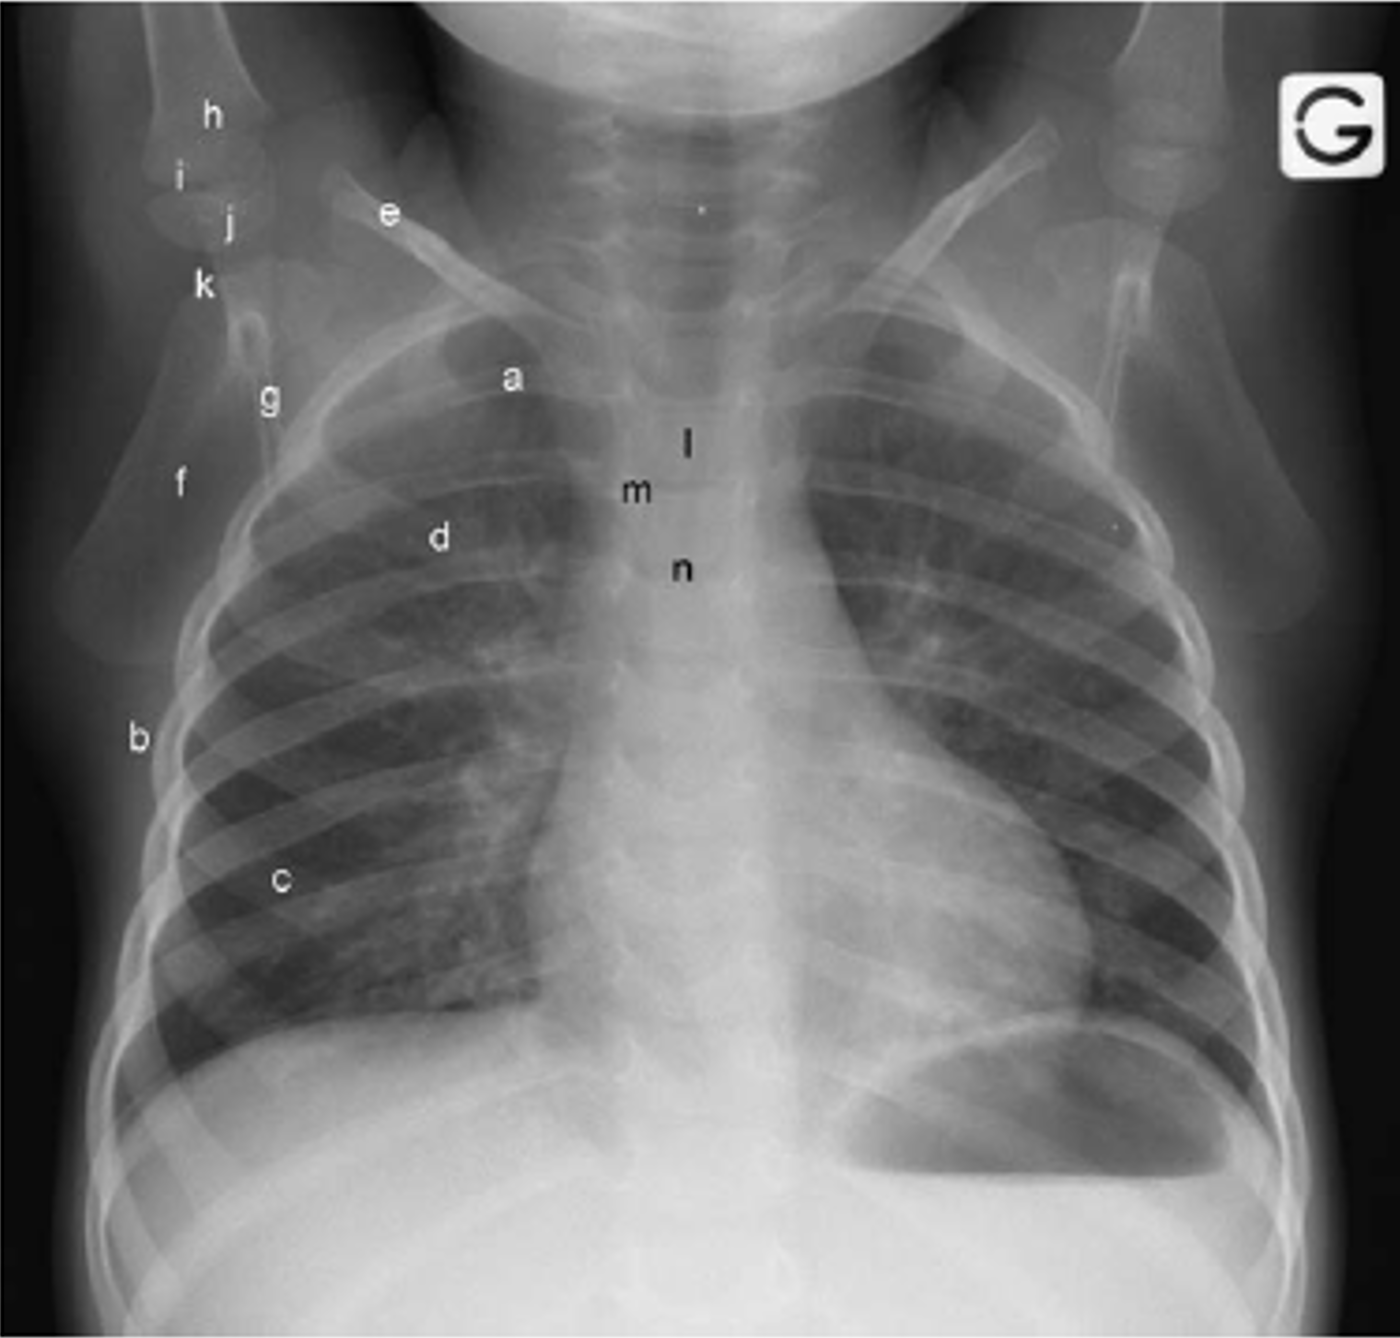
\includegraphics[width=0.4\textwidth]{thorax_osseux.png}
                \caption{Thorax osseux. a. Arc postérieur de la côte; b. arc moyen de la côte ; c. arc antérieur de la côte ; d. extrémité antérieure de la côte; e. clavicule vue en enfilade avec nouure centrale (bras relevés); f. omoplate; g. épine de l'omoplate; h. métaphyse humérale ; i. cartilage de conjugaison; j. épiphyse humérale ; k. cavité glénoïde; l. corps vertébral; m. pédicules; n. disque intervertébral.
                }\label{fig:thorax}
            \end{figure}
           
            \begin{figure}[H]
                \centering
                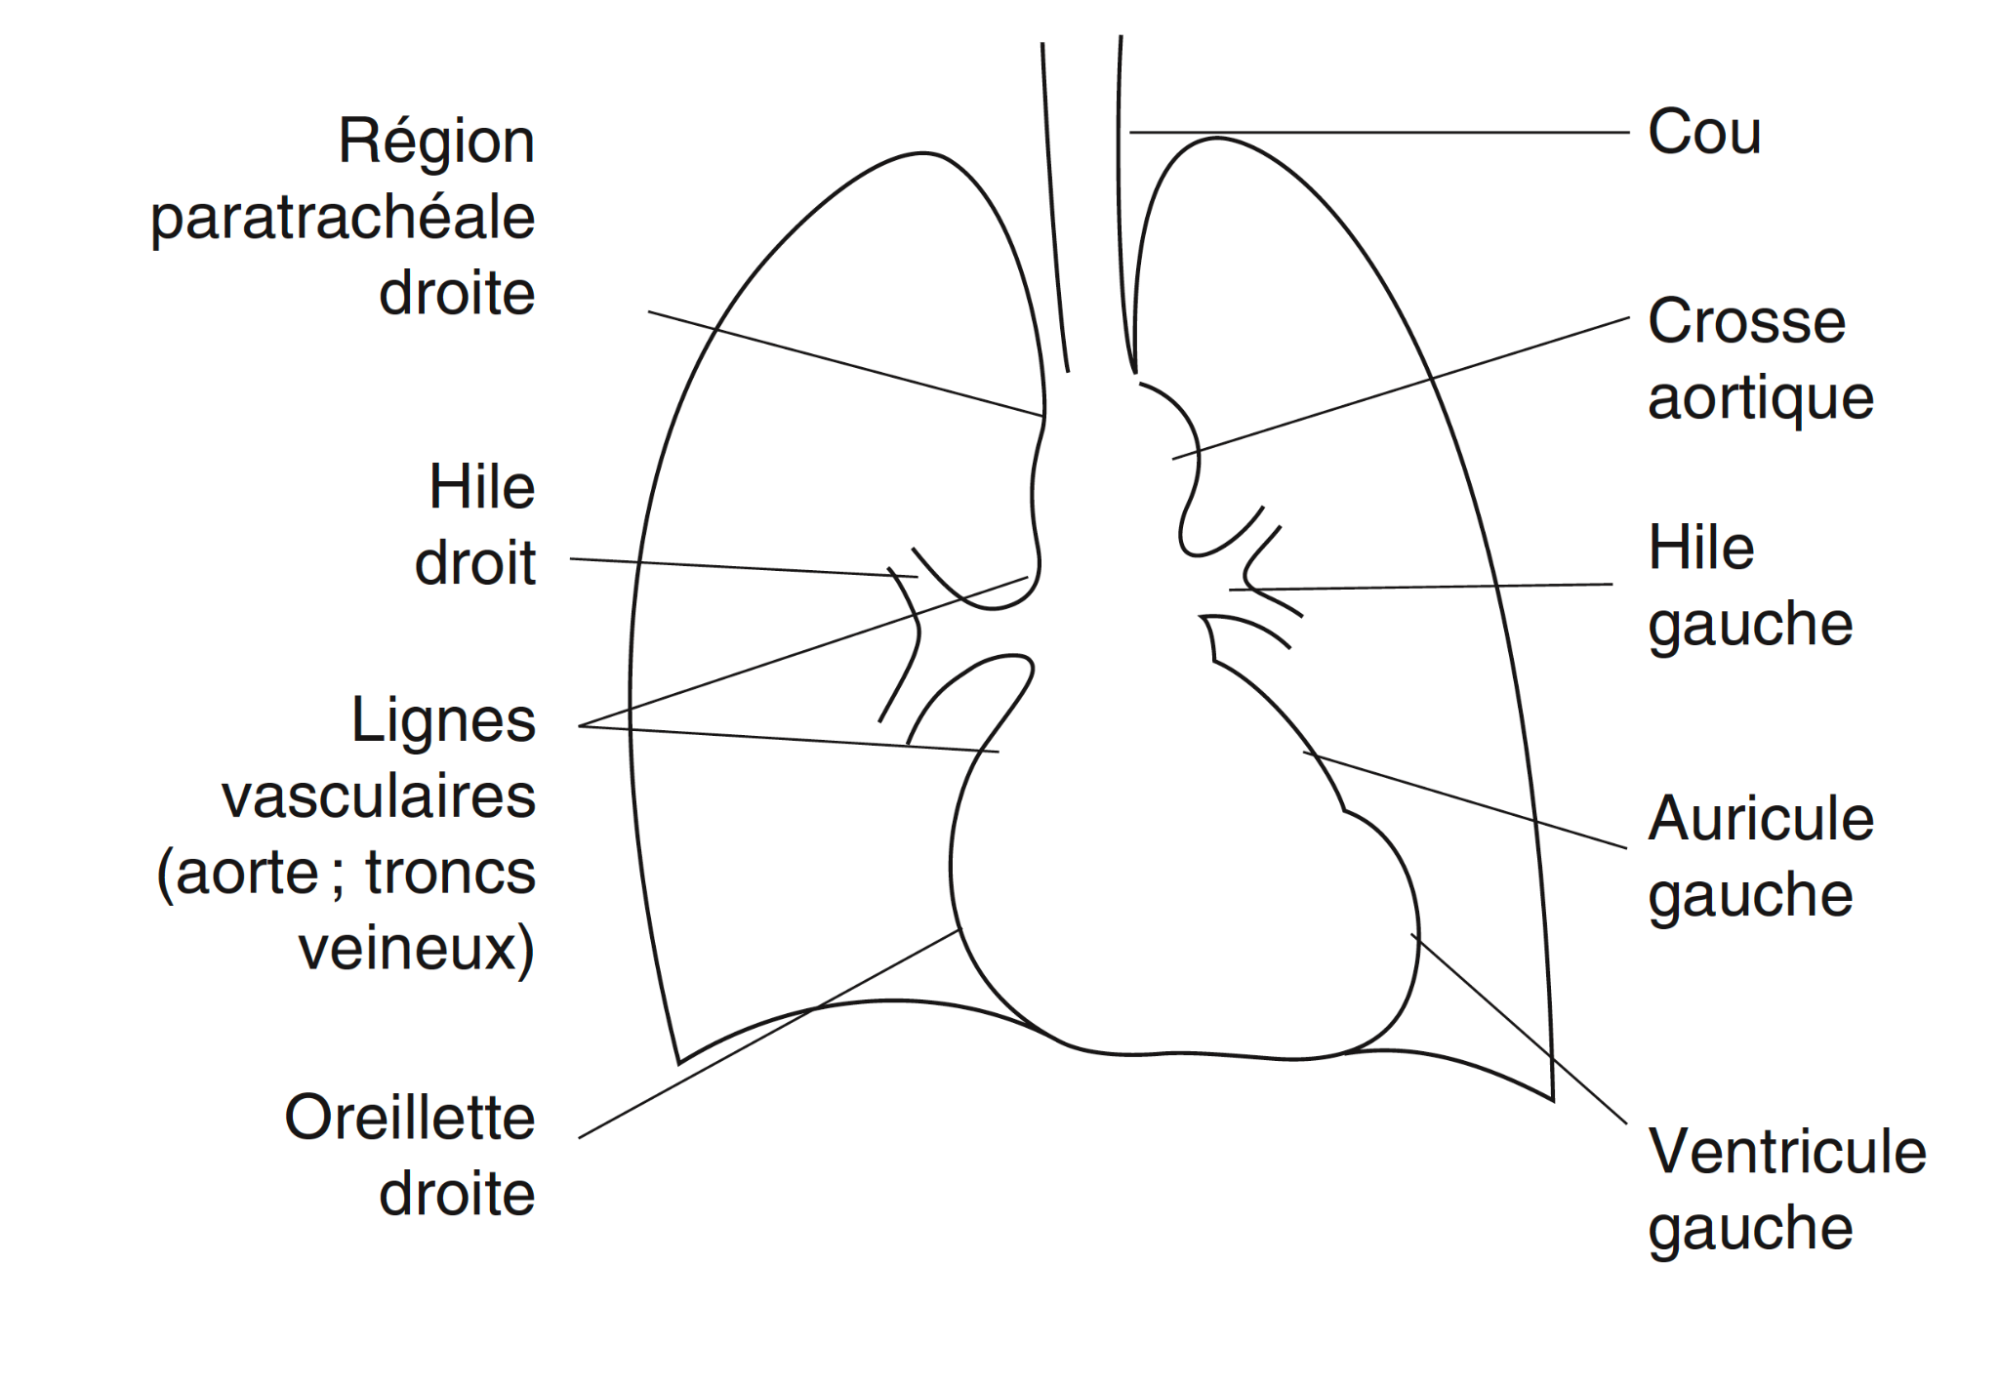
\includegraphics[width=0.6\textwidth]{dia_mediastinal.png}
                \caption{Diagramme des structures médiastinales à analyser sur une Radiographie thoracique PA}\label{fig:mediastinal}
            \end{figure}
            \subsubsection{Les differences radio anatomiques entre les clichés pédiatriques et adultes}

            Sept différences entre la radiographie thoracique d'un nourrisson et celle d'un adulte.

            \begin{figure}[H]
                \centering
                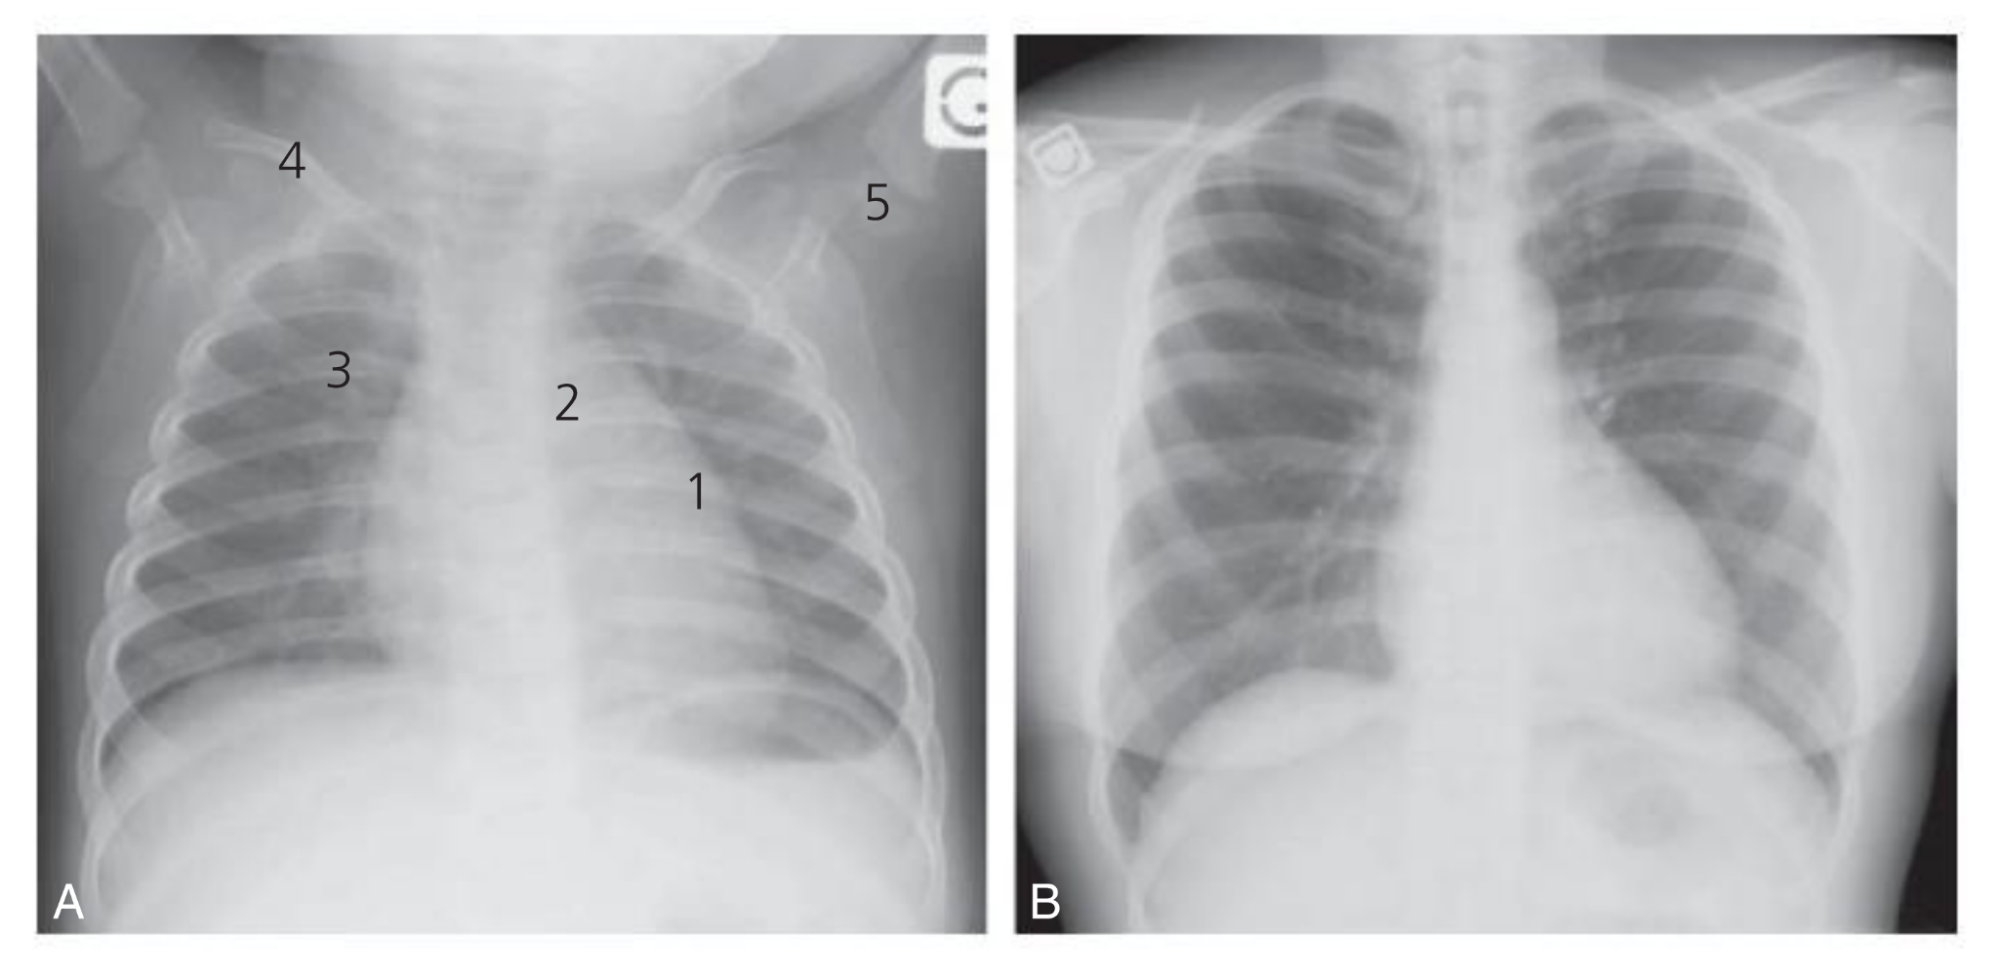
\includegraphics[width=0.6\textwidth]{differences.png}
                \caption{Les différences radio-anatomiques entre l’adult et l’enfant}\label{fig:differences}
            \end{figure}

            \begin{enumerate}
                \item présence du thymus:
                \begin{figure}[H]
                    \centering
                    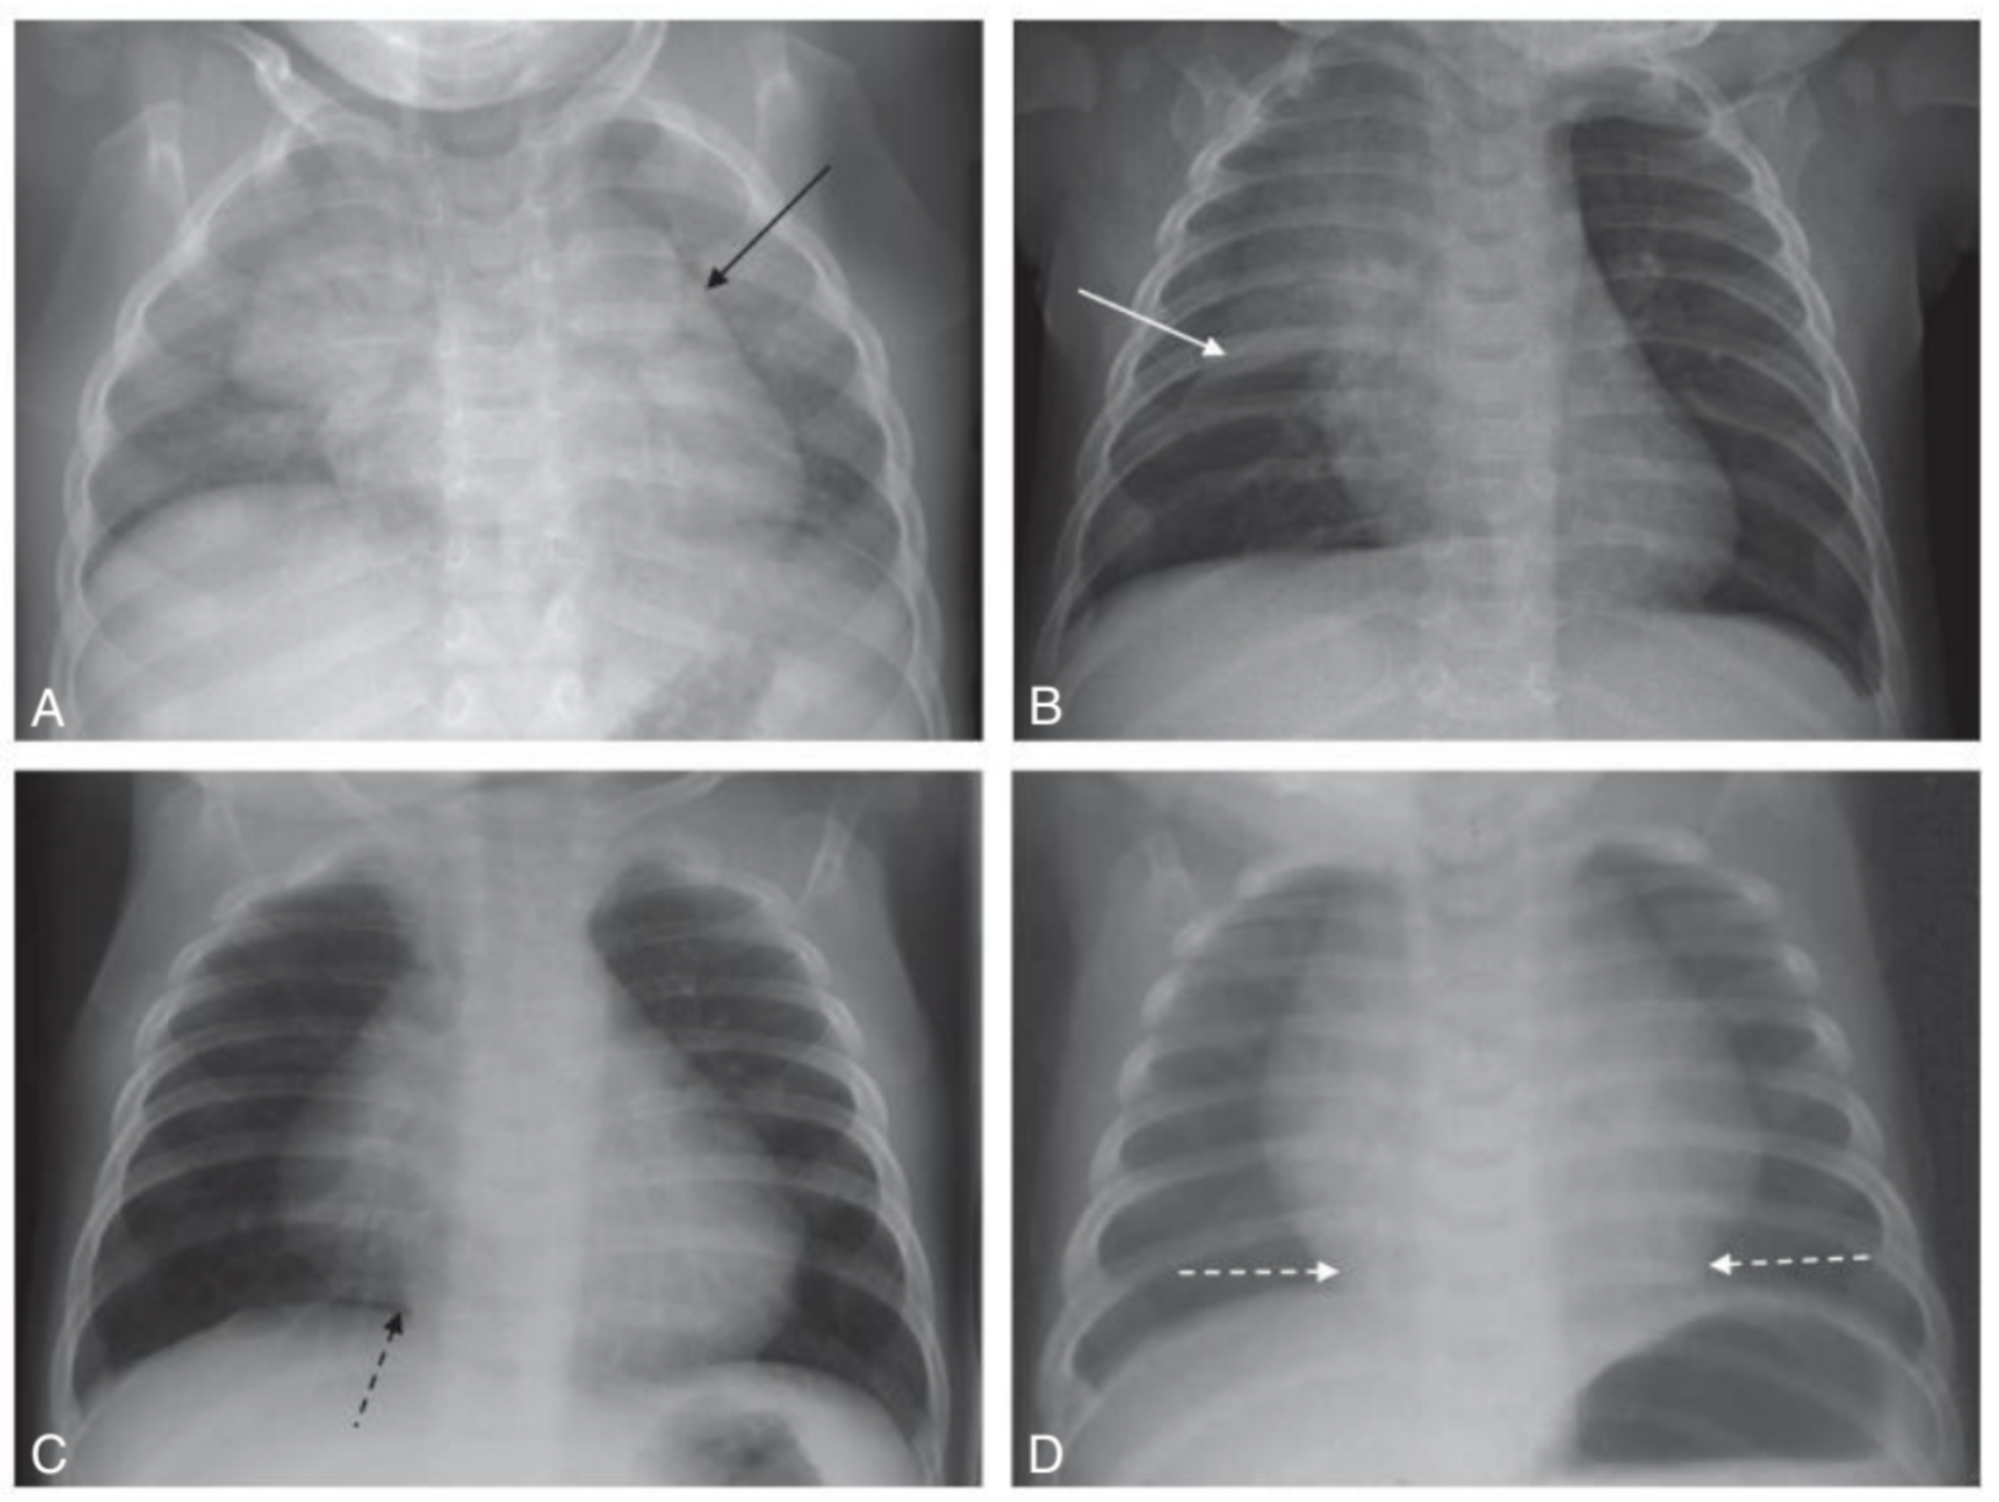
\includegraphics[width=0.6\textwidth]{thymus_enfant.png}
                    \caption{Les variations de l’image du thymus chez l’enfant}\label{fig:thymus}
                \end{figure}
                Aspects radiographiques normaux du thymus : aspect ondulé des bords du thymus sur un cliché réalisé en expiration (flèche noire) (A),aspect en voile latine (flèche blanche) (B), extension du thymus jusqu'à la coupole diaphragmatique (flèche noire en pointillés) (C),fausse impression de cardiomégalie du fait de l'extension inférieure du thymus (flèches blanches en pointillés) (D).	
                \item non visibilité du crosse aortique.
                \item portion antérieure du gril costal entièrement cartilagineuse, donc non visible sur la radiographie.
                \item courbure claviculaire accentuée du fait de la position des bras au-dessus de la tête.
                \item point d'ossification huméral supérieur.
                \item Déviation trachéale:
                \begin{figure}[H]
                    \centering
                    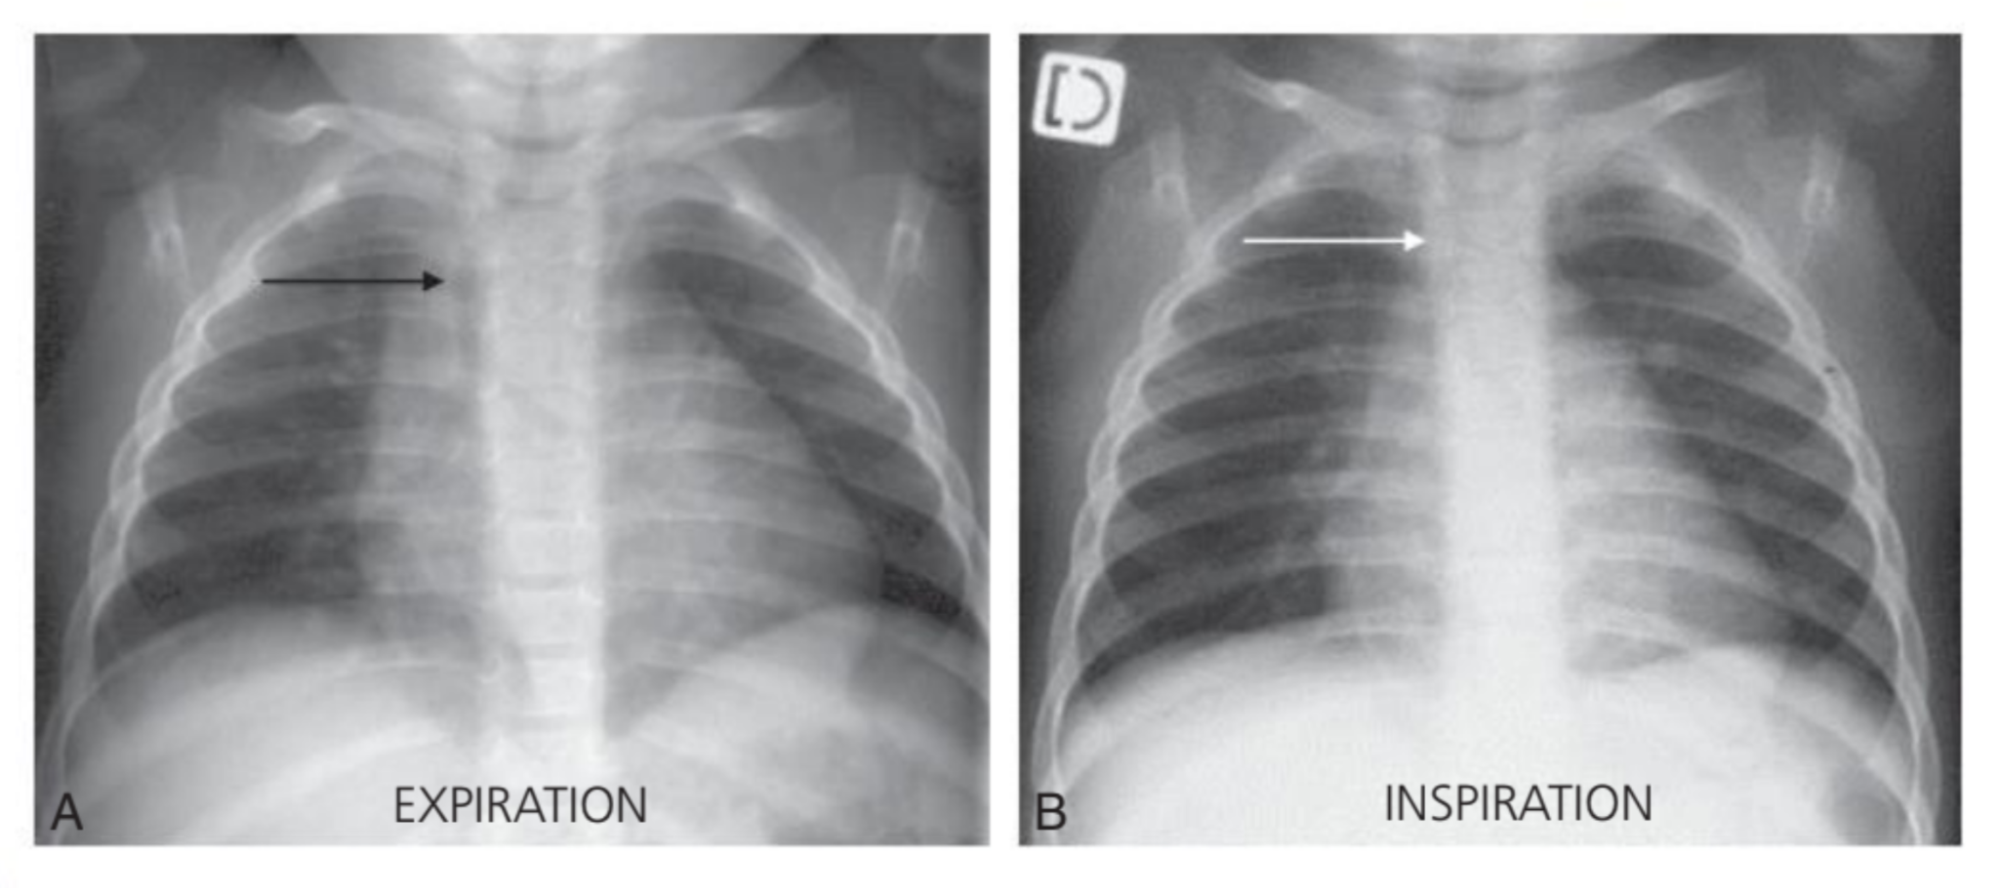
\includegraphics[width=0.6\textwidth]{tracheal.png}
                    \caption{La deviation trachéale}\label{fig:tracheal}
                \end{figure}
                Déviation trachéale physiologique vers la droite chez un nourrisson de 20 mois sur une radiographie de thorax réalisée en expiration (flèche noire) (A). Sur le cliché en inspiration, la trachée redevient rectiligne (flèche blanche) (B).
                \item L'incidence:\newline
                L'incidence de face en inspiration est suffisante dans la majorité des cas.
                Chez le petit enfant, elle est réalisée en incidence antéro-postérieure, puis en incidence postéro-antérieure lorsque l'enfant devient coopérant (après 4 ans environ).
                Chez le nouveau-né et le petit nourrisson ne tenant pas assis, l'examen est réalisé en décubitus dorsal.

            \end{enumerate}

            \subsubsection{La partie informatique de la problématique}\label{partie_info}
            Dans notre projet on veut créer un produit qui pourrait atténuer le flot des clichés thoraco-pulmonaire qui doit être traitée individuellement par les radiologues, et en particulièrement les radiographies pédiatriques qui n’ont pas assez d’attention que les radiographies adulte, mais suivant une liste des anomalies prédéfinie ou plutôt imposée par les bases données publiques à l’utilisation des étudiants, la liste des anomalies et la suivante:
            
            étudiants, et ce qui suit :
                \begin{multicols}{2}\label{list_dia}
                    \begin{enumerate}
                        \item Aucun résultat
                        \item Élargissement cardio-médiastinal
                        \item Cardiomégalie
                        \item Opacité pulmonaire
                        \item Lésion pulmonaire
                        \item Œdème
                        \item Consolidation
                        \item Pneumonie
                        \item Atélectasie
                        \item Pneumothorax
                        \item Épanchement pleural
                        \item Autre lésions pleurales 
                        \item Fracture
                        \item Appareils de soutien
                    \end{enumerate}
                \end{multicols}

                Pour plus de detail sur la liste des anomalies voir la sous-section \ref{chexpertDB}.

        \subsection{Etat d'art}
            \subsubsection{Modèles de détection automatiques de pathologies thoraciques précise chez l‘adulte}
            La dernière décennie a vu la réalisation de plusieurs applications de l'IA sur la radiographie standard et plus particulièrement la radiographie thoracique, notamment chez l'adulte.
            Ces applications ont inclus 
            
            soit la détection automatique de motifs en relation avec des anomalies thoraco-pulmonaires par exemples les études suivantes:
            
            soit la détection de pathologies thoraco-pulmonaires précises telles que:
            
            \begin{itemize}[label=$\bullet$]
                \item La détection des lésions tuberculeuses pulmonaires
                \hspace*{1cm}Les algorithmes d'IA peuvent être des outils de triage très précis et utiles pour la détection de la tuberculose dans les régions à forte prévalence.
                \item La détection précoce des lésions du cancer du poumon
                \hspace*{1cm}L'algorithme d'IA peut améliorer les performances des lecteurs pour la détection des cancers du poumon sur les radiographies pulmonaires lorsqu'il est utilisé comme second lecteur.
                \item Récemment le diagnostic du SDRA et pronostic des patients atteints de COVID-19
                \hspace*{1cm}Schéma d'évaluation par radiographie pulmonaire assisté par intelligence artificielle pour COVID-19
            \end{itemize}

            \subsubsection{Modèles de détection de Pathologies précises ou d‘anomalies à la rx thoracique chez la Population Pédiatrique}

                Sur 29 ensembles de données de radiographie pulmonaire accessibles au public, 2 ensembles de données ne comprenaient que des radiographies pulmonaires pédiatriques et 7 ensembles de données comprenaient à la fois des patients pédiatriques et adultes. 

                Padash et al.ont identifié 55 articles mettant en œuvre un modèle d'IA pour l'interprétation des radiographies thoraciques pédiatriques ou des radiographies thoraciques pédiatriques et adultes. La classification des radiographies pulmonaires comme pneumonie était l'application la plus courante de l'IA, évaluée dans 65 \% des études. Bien que de nombreuses études rapportent une précision diagnostique élevée, la plupart des algorithmes n'ont pas été validés sur des ensembles de données externes.

        \subsection{Solution Proposée}\label{Solution_prop}
        Les données de la population pédiatrique sont beaucoup moins documentées que celles de la population adulte, et notamment pour les radiographies thoraciques, ce qui nous inspirait pour créer ou collecter notre propre base de données, toujours en respectant la liste des anomalies déjà citées dans la sous-section  \ref{list_dia}.
        À cette phase du projet, il est évident que nous ne serons pas en mesure de collecter un grand ensemble de données qui serait suffisant pour construire un modèle d'apprentissage en profondeur précis pour la population pédiatrique, nous nous appuierons donc sur un ensemble de données adulte existant pour commencer reproduire un modèle d'apprentissage en profondeur capable de traiter les rayons X adultes, et alors seulement, nous utiliserons l'apprentissage par transfert pour étendre le modèle adulte, en l'alimentant par les données pédiatriques collectées, pour obtenir un modèle capable de traiter les rayons X pédiatriques.
        \begin{figure}[H]
            \centering
            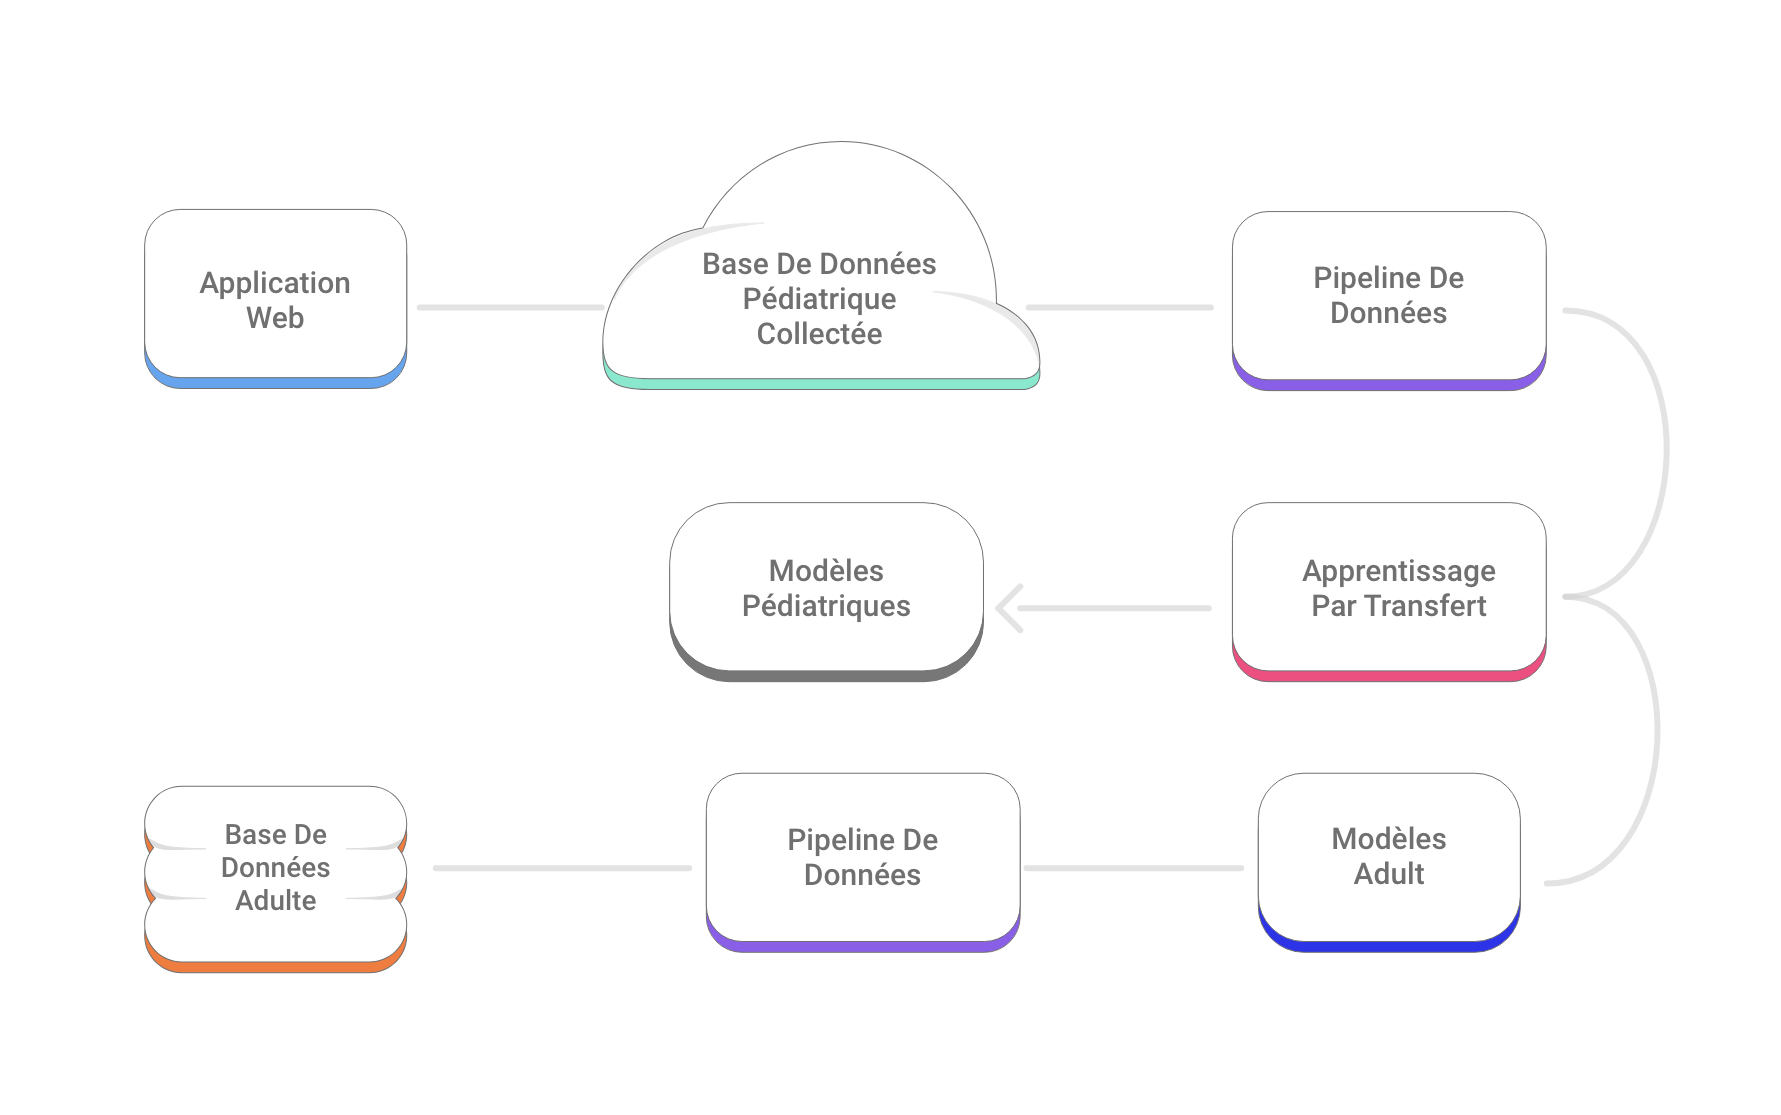
\includegraphics[width=1\textwidth]{structure_gen.jpg}
            \caption{La structure génerale de la solution proposée}\label{fig:sol_prop_01}
        \end{figure}
            \subsubsection*{Application Web}
                Premiére phase:
                Une application web qui peut collecter des données. La collecte est effectuée par les collaborateurs voir sous-section \ref{Collaborateurs}. L'application doit être simple, légère, rapide et claire avec une interface concise direct afin de ne pas prendre beaucoup de temps au médecin.
            \subsubsection*{Pipline de données}
                Deuxiéme phase:
                Étant donné que le pipeline de données sera dans une phase de pré-apprentissage, nous devons préparer une base de données bien structurée et propre où toutes les valeurs sont définies et non nulles.
            \subsubsection*{Les modeles d'apprentissage en profondeur}
                Troisiéme phase:
                Construisez des modèles d'apprentissage en profondeur qui peuvent pré-diagnostiquer les anomalies dans le thorax osseux à partio des clichés thoraciques pédiatrique.


    \section*{Conclusion}
    En conclusion, voici quelques réflexions générales sur le projet et sur ce que vous devez faire pour pouvoir créer un projet capable d'effectuer  des pré-diagnostiques des radiographies pulmonaires pédiatriques.
    \begin{enumerate}
        \item Création d'une base de données pédiatrique étiquetée suivant la liste \ref{list_dia}
        \item Création d'un pipline de données pour prétraitement des données
        \item Création des modèles d'apprentissage en profondeur
    \end{enumerate}
    Cependant, afin de poursuivre le projet, nous devons d'abord savoir ce qu'est  l'apprentissage en profondeur.
    \chapter{Apprentissage profond}

\section*{Introduction}
    Dans ce chapitre, je vais vous présenter ce qu'est le deep learning et ce que sont les réseaux de neurones, et surtout la différence entre les différentes méthodes de classification d'images.
\section{Géneralité}
    \subsection{Definition}\textbf{Deep Learning (DL):} 
            
        Selon Wikipedia L'apprentissage profond ou apprentissage en profondeur est un ensemble de méthodes d'apprentissage automatique tentant de modéliser avec un haut niveau d’abstraction des données grâce à des architectures articulées de différentes transformations non linéaires. Ces techniques ont permis des progrès importants et rapides dans les domaines de l'analyse du signal sonore ou visuel et notamment de la reconnaissance faciale, de la reconnaissance vocale, de la vision par ordinateur, du traitement automatisé du langage. Dans les années 2000, ces progrès ont suscité des investissements privés, universitaires et publics importants, notamment de la part des GAFAM (Google, Apple, Facebook, Amazon, Microsoft).
    \subsection{Historique}

    \begin{figure}[H]
        \centering
        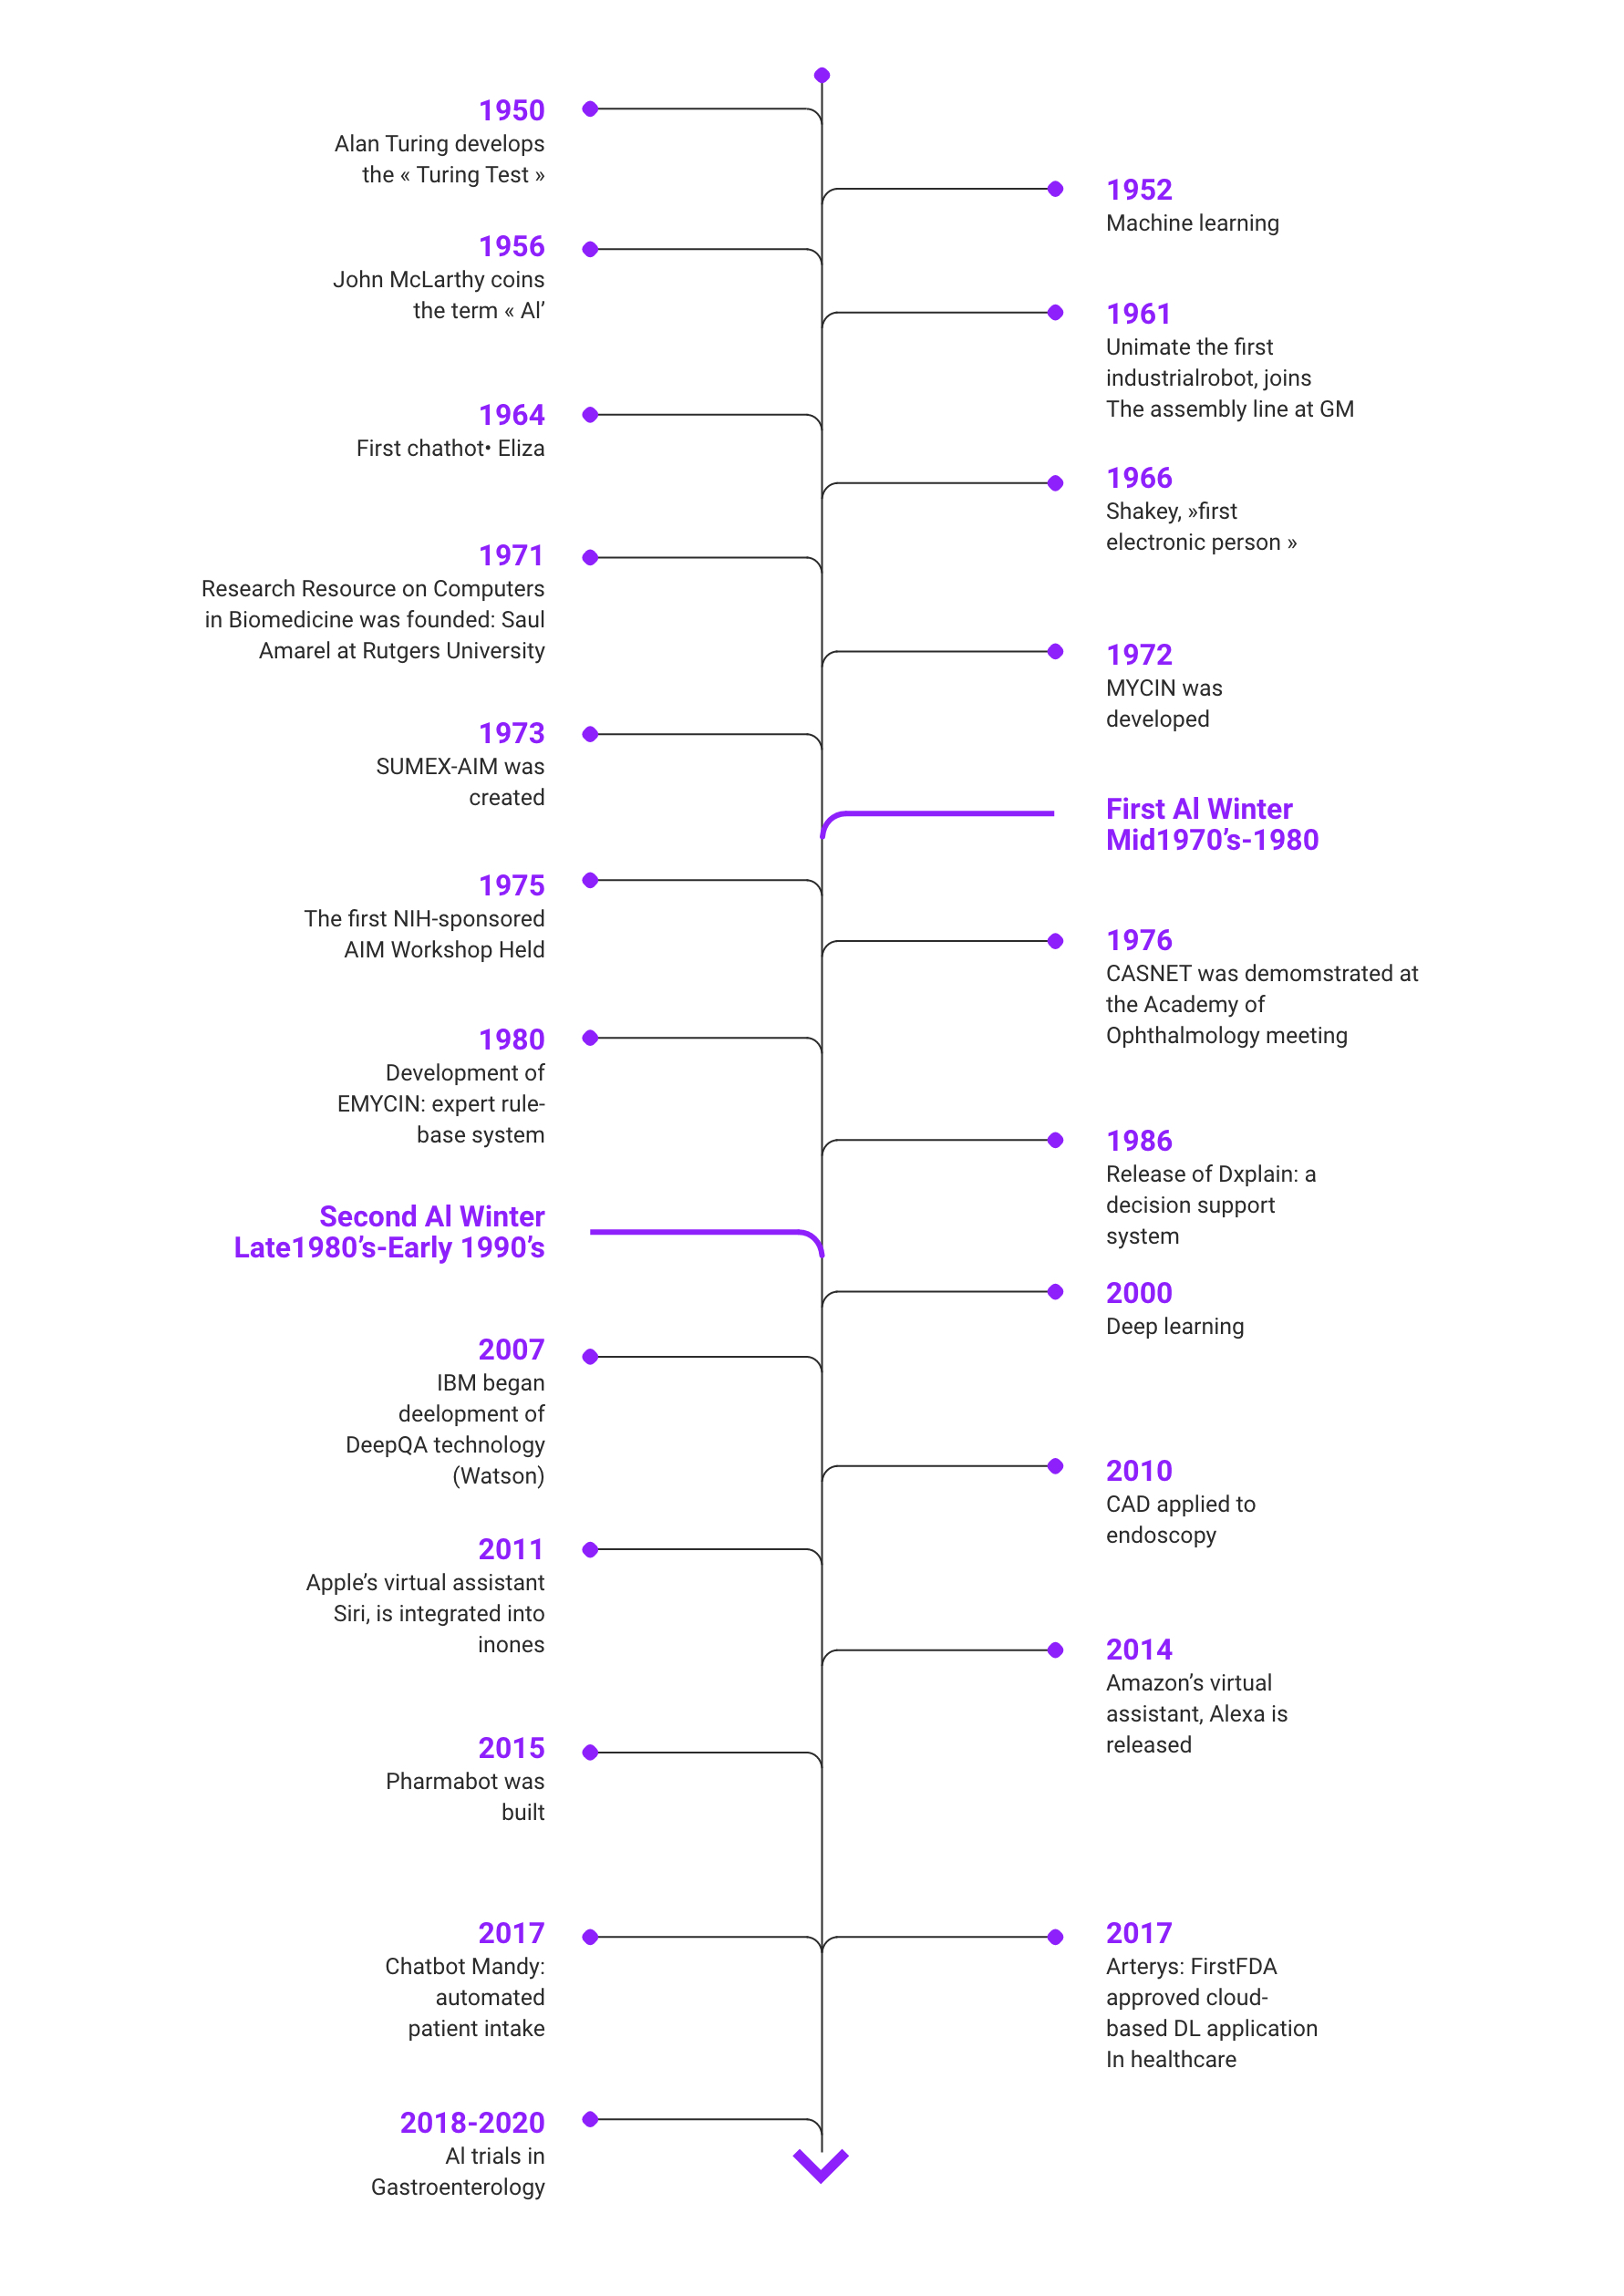
\includegraphics[width=0.8\textwidth]{history-of-ai.jpg}
        \caption{Chronologie du développement et de l'utilisation de l'intelligence artificielle en médecine. 
        À L' intelligence artificielle ; ID, apprentissage profond ; FDA, Agence fédérale américaine des produits alimentaires et médicamenteux  : CAO, diagnostic assisté par ordinateur.
        }
        \label{fig:history-of-ai}
    \end{figure}

\section{Réseau des neurones}
        un réseau de neurones est une structure qui aide l'ordinateur à imiter le processus d'apprentissage du cerveau humain, en collectant un certain nombre de nœuds liés par des poids,la manifestation la plus élémentaire d'un réseau de neurones est ce qu'on appelle le perceptron, il s'agit d'un réseau de neurones à une seule couche composé de deux entrées et d'une sortie comme suit:

        \subsection{Perceptron}
            Comme mentionné ci-dessus, le perceptron est  un lien neuronal à une seule couche avec quatre paramètres principaux. Le modèle perceptron multiplie d'abord toutes les valeurs d'entrée et leurs poids, puis ajoute ces valeurs pour créer une somme pondérée. En outre, cette somme pondérée est appliquée à la fonction d'activation "f" pour obtenir la sortie souhaitée. Cette fonction d'activation est également appelée fonction échelon et est désignée par la lettre "f".
            \begin{figure}[H]
                \centering
                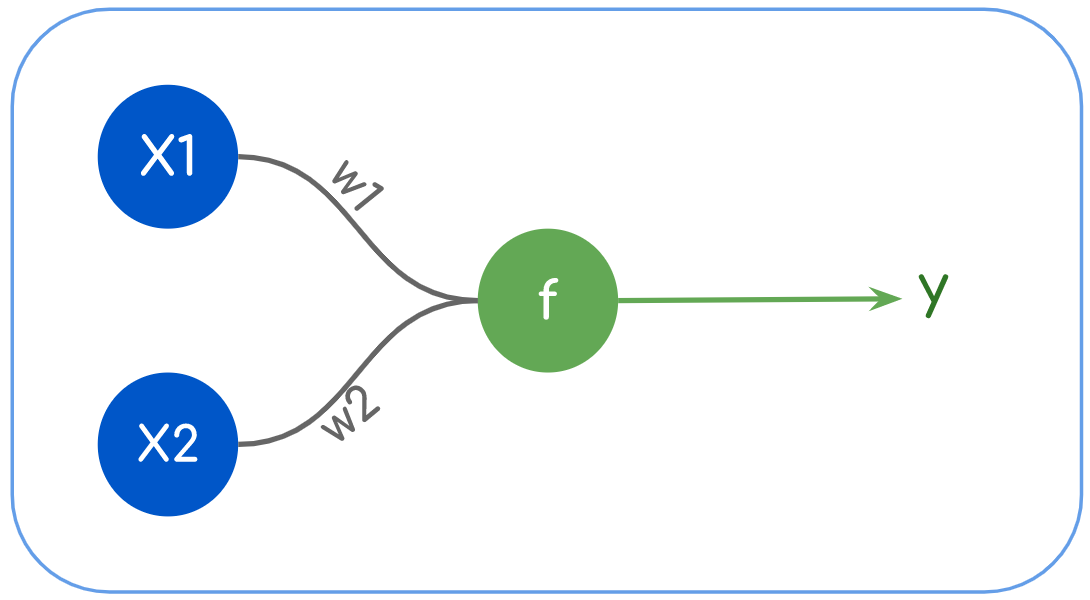
\includegraphics[scale=0.3]{perceptron}
                \caption{Perceptron}
                \label{fig:perceptron}
            \end{figure}

            \begin{itemize}[label=$\bullet$]
                \item Xi: entrées.
                \item Wi: poids.
                \item f: fonction d'activation.
                \item y: sortie 
            \end{itemize}

            cette fonction d'activation est nécessaire pour s'assurer que la sortie est  mappée entre (0,1) ou (-1,1). Notez que le poids de l'entrée indique la force d'un nœud. De même, une valeur d'entrée donne la possibilité de décaler la courbe de la fonction d'activation vers le haut ou vers le bas.
            
            Étape 1: Calculez la somme pondérée en multipliant toutes les valeurs d'entrée par leurs valeurs de poids respectives et en les additionnant. La formule est:

            \begin{equation}\label{eq:per_sum}
                \Sigma = \Sigma wi*xi = w1*x1 + w2*x2 + w3*x3 + \dots
            \end{equation}
            \myequations{Somme pondérée des entrées par leur poids}


            Nous ajoutons un terme appelé biais « b » à cette somme pondérée pour améliorer les performances du modèle. 
            Étape 2: La fonction d'activation est appliquée à l'aide des sommes pondérées ci-dessus pour donner la sortie sous forme binaire ou des valeurs continues comme suit:


            \begin{equation}\label{eq:per_func}
                Y = f(\Sigma + b)
            \end{equation}
            \myequations{Calcule de sortie}

            Étape 3: finalement pour améliorer la précision du perceptron il faut ajuster les poids suivants la relation:

            \begin{equation}\label{eq:per_weights}
                W_n = W_a + \alpha (y_r - Y) X
            \end{equation}
            \myequations{Equation de calcule des nouveaux poids}
            

            Avec \boldmath{\(W_n\)} le nouveau vecteur des poids, \textbf{\(W_a\)} le dernier vecteur de poids, \textbf{\(\alpha\)} est le pas d'apprentissage, \textbf{\(y_r\)} la sortie attendée (réele), \textbf{Y} est la sortie prévue par le perceptron et finalement \textbf{X} est le vecteur contenant les valeur courants des entrée.

        En bref, un réseau neuronal profond est une structure compliquée composée de plusieurs perceptrons interconnectés. Dans un réseau neuronal, nous avons trois unités principales, la couche d'entrée, la couche de sortie et la couche cachée contenant plusieurs couches interconnectées.
        
        \begin{figure}[H] 
            \centering
            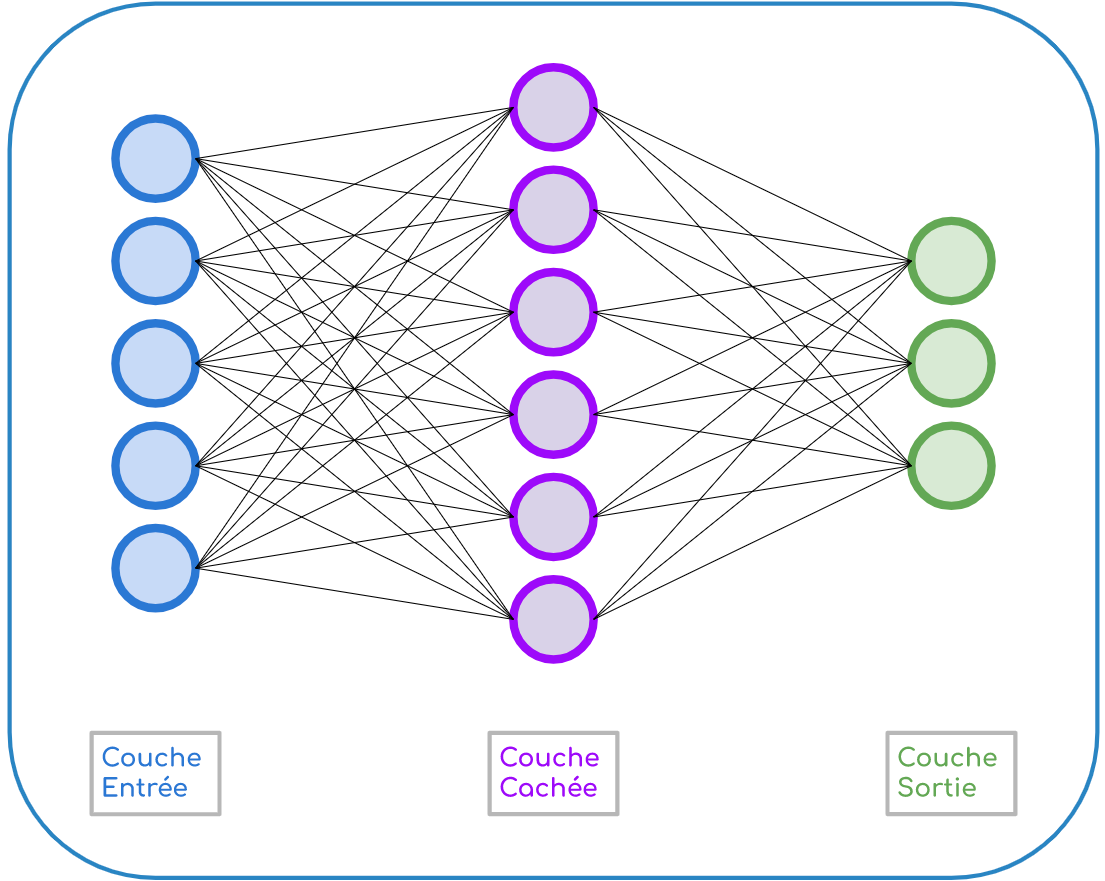
\includegraphics[width=0.8\textwidth]{multi_layer_perce.png}
            \caption{multi couche perceptron}
            \label{fig:m_l_p}
        \end{figure}

    \subsection{Réseau de neurones convolutionnel (RNC)}
    En apprentissage automatique, un réseau de neurones convolutifs (CNN ou ConvNet) est un type de réseau de neurones artificiels acycliques (feedforward) dont les schémas de connectivité entre les neurones sont inspirés du cortex visuel des animaux. Les neurones de cette zone du cerveau sont disposés pour correspondre à des zones qui se chevauchent lorsque le champ visuel est carrelé. Leur fonctionnalité s'inspire des processus biologiques et consiste en un empilement multicouche de perceptrons destiné à prétraiter de petites quantités d'informations. Les réseaux de neurones convolutifs ont un large éventail d'applications, notamment la reconnaissance d'images et de vidéos, les systèmes de recommandation et le traitement du langage naturel.

        \subsubsection{Architecture RNC standard}
        La forme la plus courante d'architecture de réseau neuronal convolutif empile plusieurs couches Conv-ReLU, suivies de couches de pool supplémentaires, répétant ce modèle jusqu'à ce que l'entrée soit réduite à un espace  suffisamment petit. À un moment donné, il est courant de mettre une couche entièrement connectée (FC). La dernière couche entièrement connectée sera connectée à la sortie. Vous trouverez ci-dessous une architecture de réseau neuronal convolutif commune qui suit ce modèle:

        \begin{figure}[H] 
            \centering
            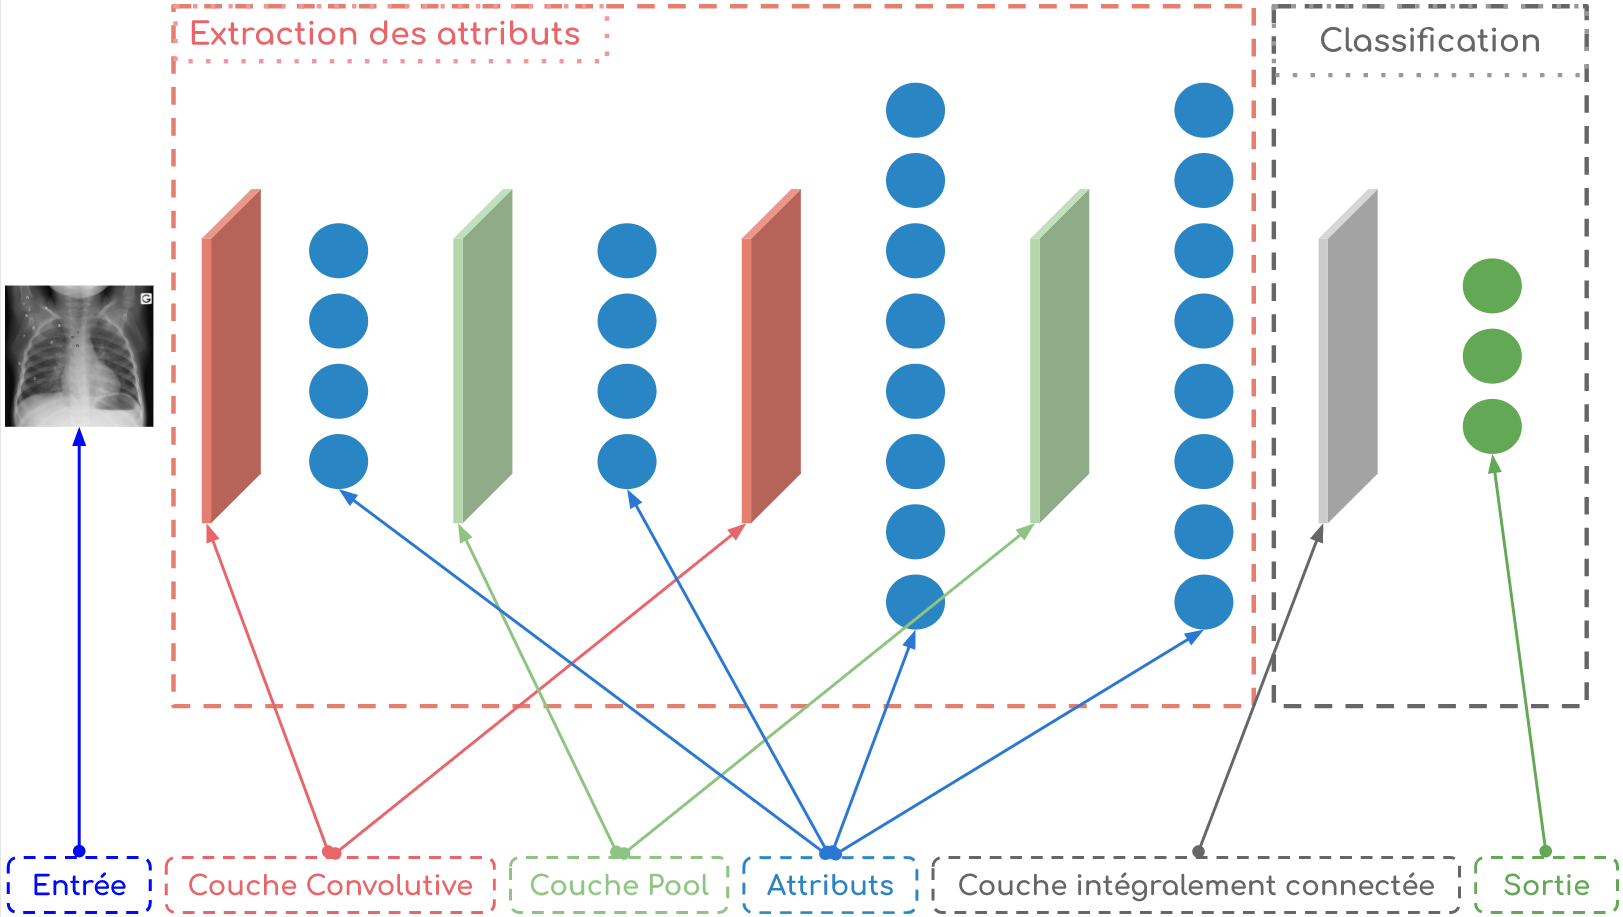
\includegraphics[width=\textwidth]{conv_stand_arch.png}
            \caption{Architecture standard d'un Réseau de neurones convolutionnel}
            \label{fig:conv_stand_arch}
        \end{figure}

        \subsubsection{Couche convolutive}
        Les couches convolutives sont à la base des CNN. Un paramètre de tranche consiste en un ensemble de filtres d'apprentissage (ou noyaux). Ces filtres ont un petit champ de vision, mais couvrent toute la profondeur du volume d'entrée. Dans le (Feed forward), chaque filtre est convolué sur la largeur et la hauteur du volume d'entrée et le produit scalaire entre les entrées du filtre est calculé pour produire la carte d'activation 2D pour ce filtre. Par conséquent, le réseau apprend quels filtres s'activent lorsqu'il détecte certains types d'entités à certains emplacements spatiaux dans l'entrée. 
        L'empilement des cartes d'activation de tous les filtres le long de la dimension de profondeur forme le volume de sortie complet de la couche de convolution. Chaque entrée dans le volume de sortie peut donc également être interprétée comme la sortie d'un neurone partageant des paramètres avec des neurones dans la même carte d'activation en regardant une petite région à l'intérieur de l'entrée.

        \subsubsection{Couche max pooling}
        Une couche max pooling est une nouvelle couche ajoutée après la couche de convolution. Surtout après avoir appliqué des non-linéarités (telles que ReLU)  aux cartes de caractéristiques générées par les couches convolutionnelles. 
        L'ajout d'une couche de max pooling après une couche convolutive est un modèle courant utilisé pour ordonner les couches dans les réseaux de neurones convolutifs qui se répètent une ou plusieurs fois dans un modèle particulier. 
        La couche max pooling fonctionne sur chaque carte d'entités indépendamment, créant un nouvel ensemble du même nombre de cartes d'entités regroupées.

        
        \subsubsection{Hyperparamètres}
        En apprentissage automatique, les hyperparamètres sont des paramètres dont les valeurs sont utilisées pour contrôler le processus d'apprentissage. En revanche, les valeurs des autres paramètres (généralement les poids des nœuds) sont obtenues par apprentissage. 
        Les hyperparamètres peuvent être classés comme des hyperparamètres de modèle qui ne peuvent pas être dérivés en ajustant une machine à un ensemble d'apprentissage, ou des hyperparamètres de modèle, car ils s'appliquent à la tâche de sélection de  modèle. Algorithmes qui, en principe, n'affectent pas les performances du modèle, mais affectent la vitesse et la qualité du processus d'apprentissage. Des exemples d'hyperparamètres de modèle sont la topologie et la taille du réseau neuronal. Des exemples d'hyperparamètres algorithmiques sont le taux d'apprentissage et la taille de la pile.
        \paragraph{Choix des hyperparamètres}
        Les réseaux de neurones convolutifs utilisent plus d'hyperparamètres que les perceptrons multicouches standards. Même si les règles habituelles de taux d'apprentissage et de constantes de régularisation s'appliquent toujours, les notions de nombre de filtres, leur forme et la forme du max pooling doivent être prises en considération.




\section{Classification des images}
    La classification des images est une tâche fondamentale qui tente de comprendre l'image dans son ensemble. Le but est de classer les images en leur attribuant des étiquettes spécifiques. La classification des images fait généralement référence aux images dans lesquelles un seul objet est affiché et  analysé. En revanche, la détection d'objets comprend à la fois des tâches de classification et de localisation et est utilisée pour analyser des cas plus réalistes où plusieurs objets peuvent être présents dans une image.

    Dans le domaine de la classification des images, nous avons exploré trois types bien connus:
    \begin{enumerate}
        \item Classification binaire
        \item Classification Multi-Classes
        \item Classification Multi-Etiquettes
    \end{enumerate}

    \subsection{Classification binaire}
        La classification binaire fait référence aux tâches de classification avec deux étiquettes de classe. 
        Les tâches de classification binaire ont généralement une classe représentant les conditions normales et une autre classe représentant les conditions anormales. 
        Et dans notre cas, dans l'image, on fait référence à la présence d'objets (en prenant l'étiquette 0) ou non (en prenant l'étiquette 1).
    \subsection{Classification Multi-Classes}
        Contrairement à la classification binaire, la classification multi-classes n'a pas la notion de résultats normaux et anormaux. Au lieu de cela, les exemples sont classés comme appartenant à l'une parmi une gamme de classes connues.

        Le nombre d'étiquettes de classe peut être très important sur certains problèmes. Par exemple, un modèle peut prédire qu'une photo appartient à un parmi des milliers ou des dizaines de milliers de visages dans un système de reconnaissance faciale.

        Mais la chose la plus importante à noter est que le résultat prédit de ce modèle est une classe unique qui le rend moins intéressant dans notre cas où une radiographie peut avoir de multiples anomalies.
    \subsection{Classification Multi-Etiquettes}
        Ceci est différent de la classification binaire ou multiclasse, où une seule étiquette de classe est prédite par instance. 
        Il est courant de modéliser des tâches de classification multi-étiquettes à l'aide de modèles qui prédisent plusieurs sorties, où chaque sortie est prédite sous la forme d'une distribution de probabilité de Bernoulli. Il s'agit essentiellement d'un modèle qui effectue plusieurs prédictions de classification binaire par exemple. 
        Les algorithmes de classification utilisés pour la classification binaire ou multiclasse ne peuvent pas être utilisés directement pour la classification multiétiquette. Une version spéciale de l'algorithme de classification standard est disponible, appelée version multi-étiquettes de l'algorithme:
        \begin{itemize}[label=$\bullet$]
            \item Arbres de décision multi-étiquettes
            \item Forêts aléatoires multi-étiquettes
            \item Amplification des dégradés multi-étiquettes
        \end{itemize}


\section{Apprentissage par transfert}
    L'apprentissage par transfert est la réutilisation de modèles pré-entraînés pour de nouveaux problèmes. Il est actuellement très populaire  en apprentissage profond car il permet d'entraîner des réseaux de neurones profonds avec relativement peu de données. Ceci est très utile dans le domaine de la science des données. En effet, la plupart des problèmes du monde réel n'ont généralement pas des millions de points de données étiquetés pour entraîner un modèle aussi complexe.


\section*{Conclusion}
        Ce qu'on peut en deduire de ce chapitre c'est que pour la réussite de notre projet on doit se baser sur 3 concept principales:
        \begin{enumerate}
            \item Réseaux de neurones convolutifs
            Pour le traitement des données qui ont sous forme de clichés de radiologiques (images)
            \item Classification Multi-Etiquettes
            Car on veut que le modèle détecte tout les anomalies possible non seulement une.
            \item Apprentissage par transfert
            On a pas assés de données pour crée un modèle puissant donc on va se baser sur un modèle pré-entraîné, pour assurer une bon précision avec le minimum de données.
        \end{enumerate}
    \chapter{Etude technique}

\section*{Introduction}
La conception et la modélisation sont à la base du projet. Les connaître nous permettra de bien définir les autres composantes et besoins de ce projet. Cela comprend les choix techniques et les outils informatiques utilisés pour obtenir des résultats satisfaisants. C'est un projet  structuré avec des composants interconnectés pour un excellent flux de travail.

\section{Conception et modelisation}
Maintenant que nous avons décrit les phases du problème, concentrons-nous sur les phases fondamentales du cycle de vie du logiciel: les phases de conception et de modélisation. Le but de cette phase est de dériver une spécification pour l'architecture du système. 
Cette phase conduit à la conception et à la schématisation de classes et de séquences basées sur le langage de modélisation UML.

Dans tout ce qui précède, nous pouvons remarquer une structure légèrement différente de celle que nous avons déjà montrée dans la section \ref{Solution_prop}.
    \subsection{Structure générale du projet}
    Pour construire une nouvelle structure, il faut s'appuyer sur les points issus du chapitre précédent.

    Pour ce faire, on doit utiliser une base de données secondaire. Il s'agit d'une grande base de données structurée de la population adulte, pour construire des modéles pré-entraînés sur des donnéees de la population adulte, Un phénomène décidément très proche du nôtre.
    Après tous ces considérations on a trouver la structure du figure \ref{fig:structure_gen}
    \begin{figure}[H]
        \centering
        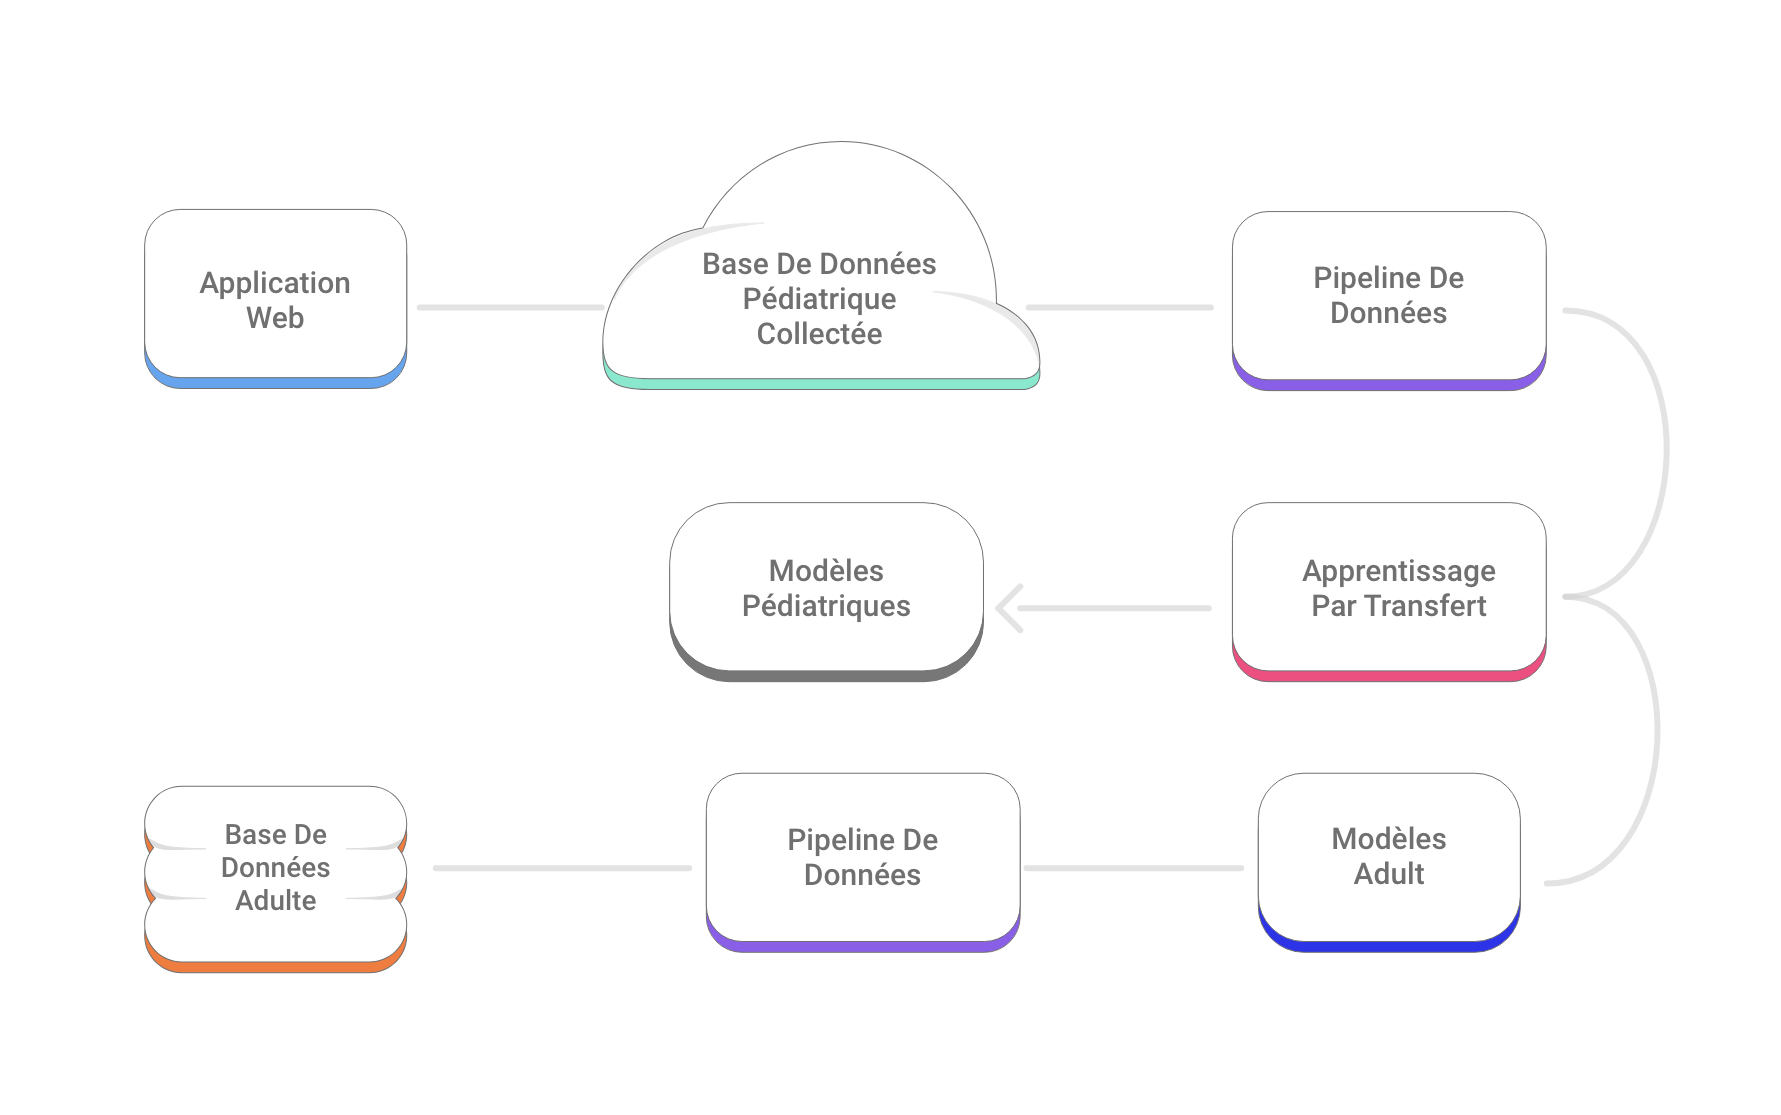
\includegraphics[width=0.7\textwidth]{structure_gen.jpg}
        \caption{structure génerale du projet}\label{fig:structure_gen}
    \end{figure}
    \subsection{Application Web}
        L'application Web est une API simple pour la collection et la visualisation de données, donc son architecture de base est également simple, c'est comme suit figure \ref{fig:xpedia_arc}
        \begin{figure}[H]
            \centering
            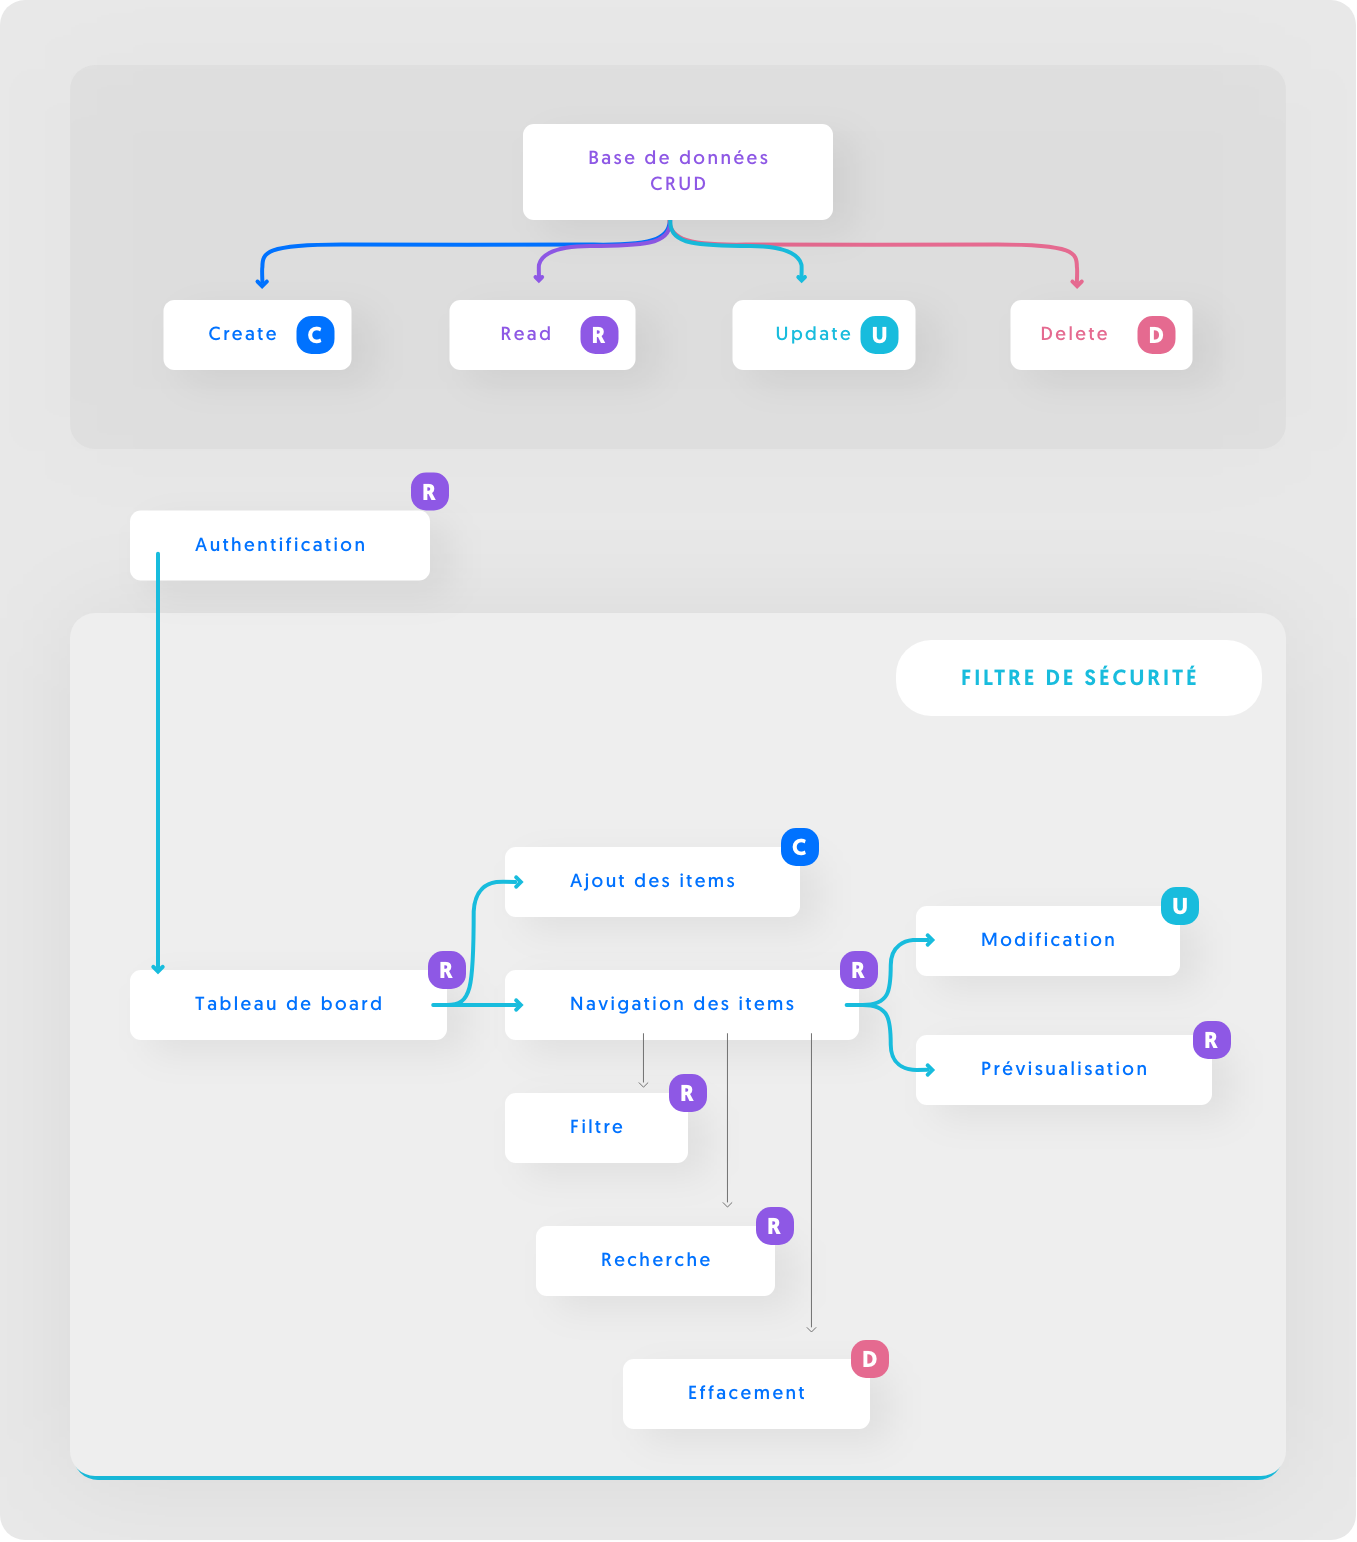
\includegraphics[width=1\textwidth]{xpedia_arc.png}
            \caption{structure génerale de l'application web Xpedia}\label{fig:xpedia_arc}
        \end{figure}
        \subsubsection{UML}
            UML (abréviation de Unified Modeling Language) est un langage de modélisation standardisé composé d'un ensemble de diagrammes intégrés qui aident les développeurs de systèmes et de logiciels à spécifier, visualiser et visualiser les artefacts des systèmes logiciels. .système. UML représente un ensemble éprouvé de meilleures pratiques techniques pour la modélisation de systèmes vastes et complexes et constitue une partie très importante du développement logiciel orienté objet et du processus de développement logiciel. UML utilise principalement une notation graphique pour représenter la conception de projets logiciels.

            \begin{enumerate}
                \item Diagramme de classe:
                Notre diagramme de classe de  deux classes utilisateur et xray (cliché), notre but de cette application et de collectés les données (xrays), l'acteur qui va effectuer la collection est l'utilisateur:
                \begin{figure}[H]
                    \centering
                    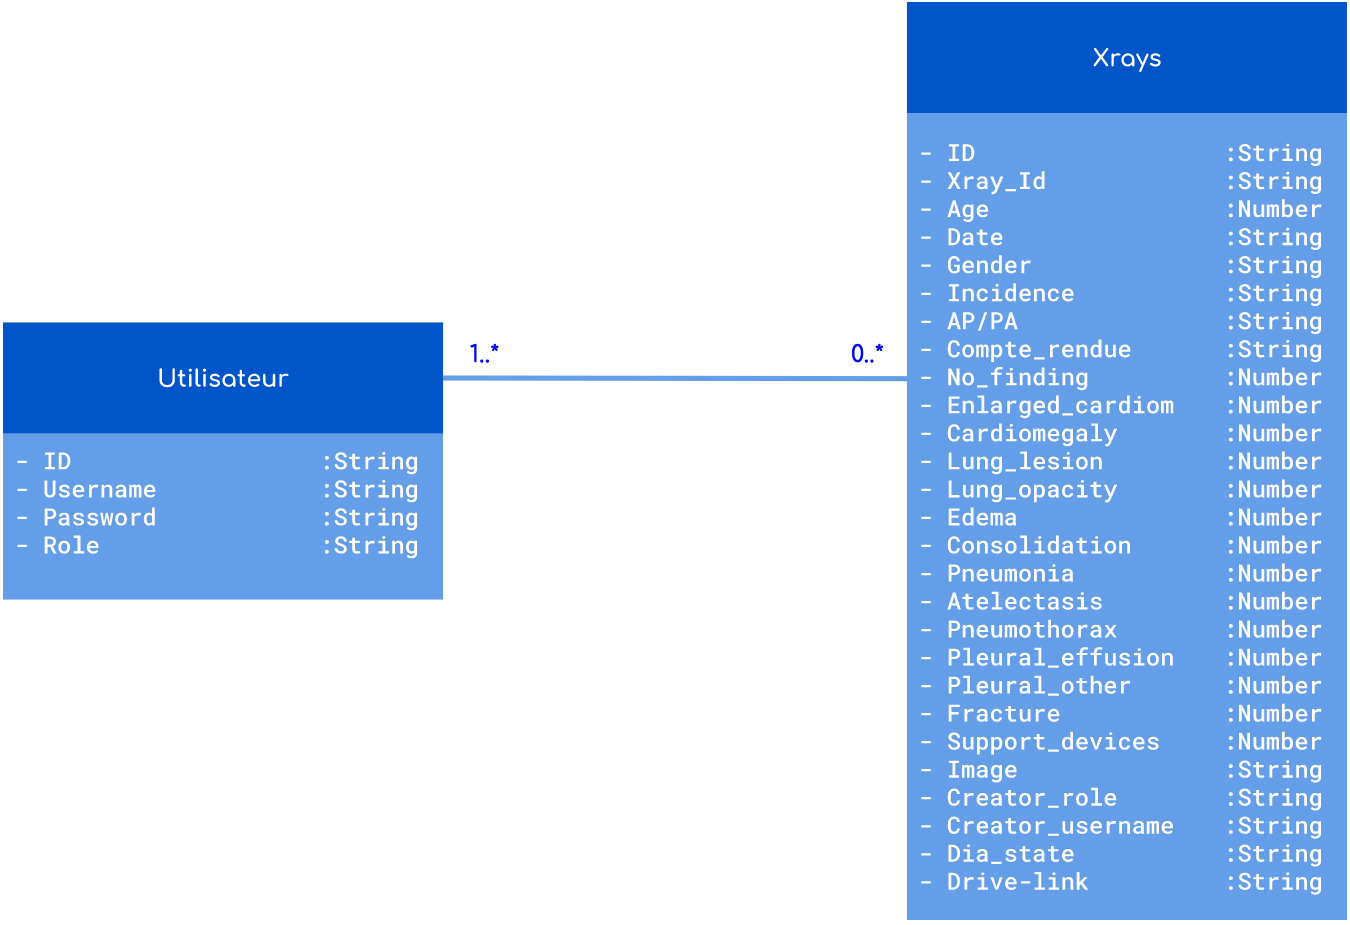
\includegraphics[width=0.8\textwidth]{class_dia.png}
                    \caption{Le diagramme de classe de l'application web Xpedia}\label{fig:class_dia}
                \end{figure}

                \item Diagrammes de séquence
                
                Un diagramme de séquence représente les objets impliqués dans une interaction particulière et les messages qu'ils échangent organisés par ordre chronologique.
                \begin{enumerate}
                    \item Diagramme de séquence: cas d'authentification
                    \begin{figure}[H]
                        \centering
                        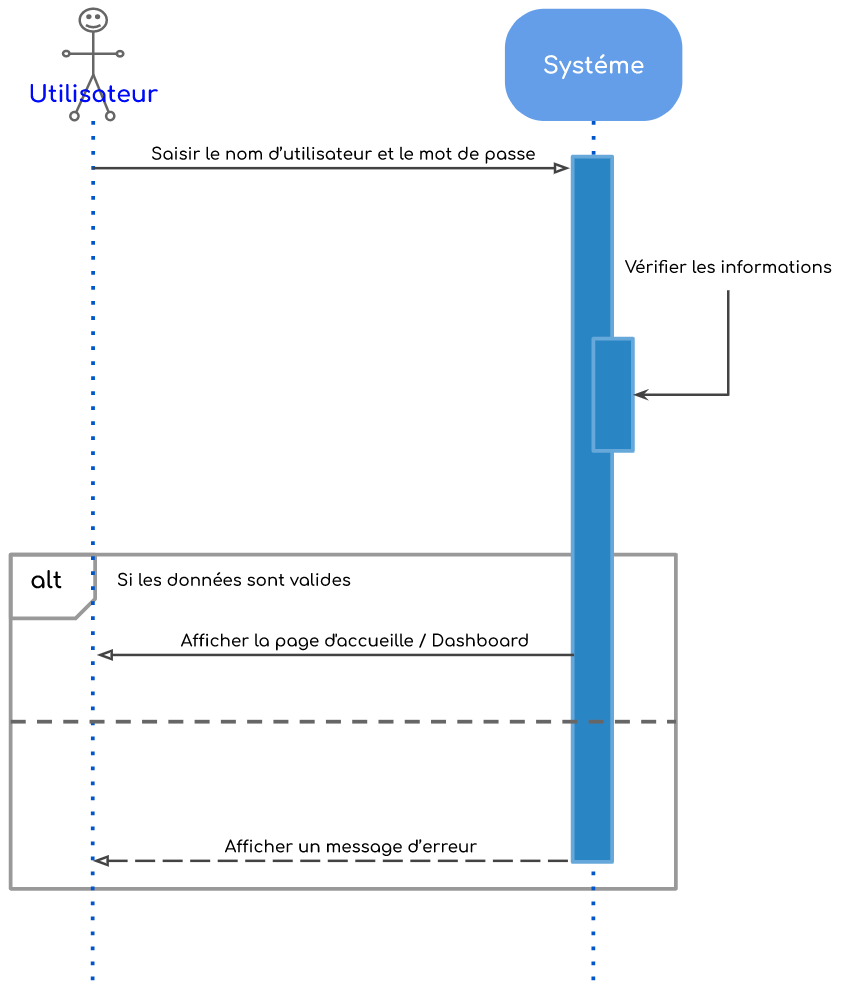
\includegraphics[width=0.5\textwidth]{cas_auth.png}
                        \caption{Le diagramme de séquence: cas d'authentification}\label{fig:cas_auth}
                    \end{figure}

                    Comme on peut le voir sur la figure \ref{fig:cas_auth}, l'authentification se fait à travers 2 opérations principales:
                    \begin{itemize}[label=$\bullet$]
                        \item l'utilisateur fournit le nom d'utilisateur et le mot de passe
                        \item le système recoupe les informations fournies avec les données existantes dans la collection de l'utilisateur
                    \end{itemize}
                    \item Diagramme de séquence: cas d'ajouter un cliché
                    \begin{figure}[H]
                        \centering
                        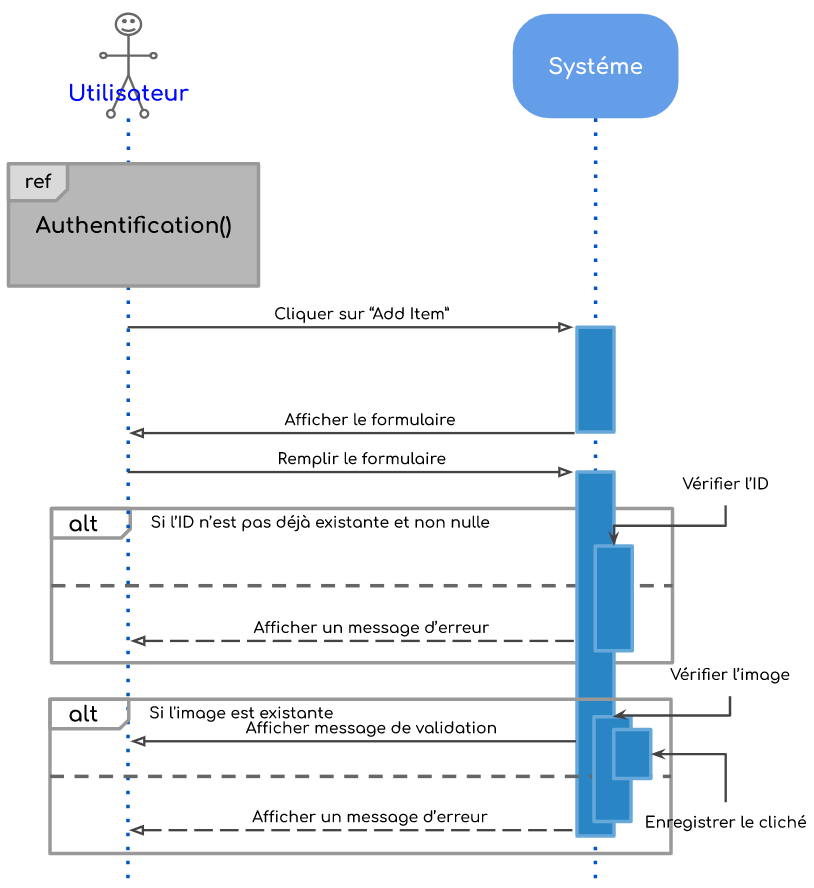
\includegraphics[width=0.5\textwidth]{cas_add.png}
                        \caption{Le diagramme de séquence: cas d'ajouter un cliché}\label{fig:cas_add}
                    \end{figure}
                \end{enumerate}
            \end{enumerate}
        
    \subsection{Pipeline de données}
    \paragraph*{Un pipeline de données est} une série d'étapes de traitement de données. Si les données ne sont pas actuellement chargées dans la plateforme de données, elles seront ingérées au début du pipeline. Ensuite, vous avez une séquence d'étapes où chaque étape fournit une sortie qui devient l'entrée de l'étape suivante. Cela continue jusqu'à ce que le pipeline soit terminé. Dans certains cas, des étapes indépendantes peuvent s'exécuter en parallèle.  
    
    Un pipeline de donnéesse compose de trois éléments principaux : une source, une ou plusieurs étapes de traitement et une destination. Dans certains pipelines de données, une destination peut être appelée un récepteur. Par exemple, un pipeline de données peut transmettre des données de votre application à un entrepôt de données, d'un lac de données à une base de données d'analyse ou à un système de traitement des paiements. Un pipeline de données peut également avoir la même source et le même récepteur, de sorte que le pipeline n'a besoin que de modifier l'ensemble de données. Chaque fois que des données sont traitées entre le point A et le point B (ou les points B, C, D), il existe un pipeline de données entre ces points.
    \begin{figure}[H]
        \centering
        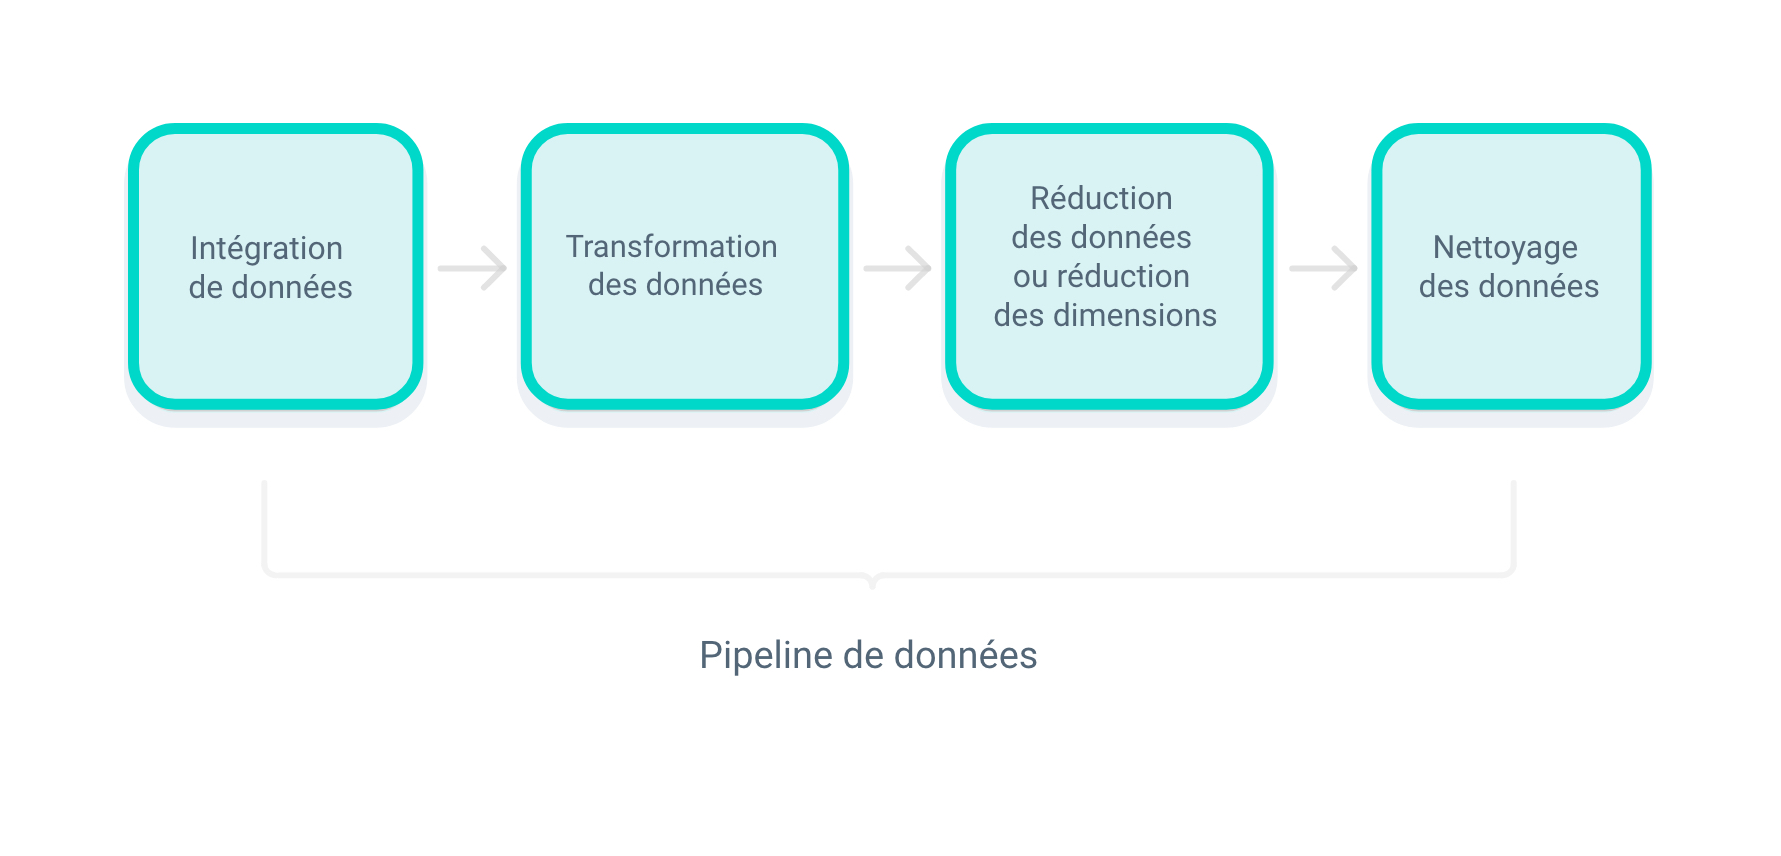
\includegraphics[width=0.8\textwidth]{data-preprocessing.jpg}
        \caption{La structure d'un pipeline de données}\label{fig:data_preprocessing}
    \end{figure}
        \subsubsection{Integration}
        L'intégration de données est le processus consistant à combiner des données provenant de différentes sources en une vue unique et unifiée. L'intégration commence par le processus d'ingestion et comprend des étapes telles que le nettoyage, le mappage ETL et la transformation. L'intégration des données permet finalement aux outils d'analyse de produire une intelligence économique efficace et exploitable.

        Il n'existe pas d'approche universelle de l'intégration des données. Cependant, les solutions d'intégration de données impliquent généralement quelques éléments communs, notamment un réseau de sources de données, un serveur maître et des clients accédant aux données à partir du serveur maître.

        Dans un processus d'intégration de données typique, le client envoie une demande de données au serveur maître. Le serveur maître reçoit ensuite les données nécessaires à partir de sources internes et externes. Les données sont extraites des sources, puis consolidées en un seul ensemble de données cohérent. Ceci est renvoyé au client pour utilisation.
        \subsubsection{Transformation}
        La transformation des données est le processus de transformation des données d'un format à un autre. Généralement, vous convertissez du format du système source au format requis par le système cible. Les transformations de  données font partie de la plupart des tâches d'intégration et de gestion des données, telles que : B. Gestion des données et stockage des données. 

        En tant qu'étape du processus ELT/ETL, la transformation des données peut être qualifiée de « simple » ou de « complexe » selon le type de modifications qui doivent être apportées aux données avant qu'elles ne soient livrées à leur destination. Le processus de transformation des données peut être effectué à l'aide de l'automatisation, de l'administration manuelle ou d'une combinaison des deux.

        \subsubsection{Réduction}
        La réduction des données signifie la réduction de certains aspects des données, généralement le volume de données. La réduction peut également porter sur d'autres aspects tels que la dimensionnalité des données lorsque les données sont multidimensionnelles. La réduction de tout aspect des données implique généralement une réduction du volume de données.

        La réduction des données n'a de sens en soi que si elle est associée à une certaine finalité. Le but à son tour dicte les exigences pour les techniques de réduction de données correspondantes. Un but naïf de la réduction des données est de réduire l'espace de stockage. Cela nécessite une technique pour compresser les données dans un format plus compact et également pour restaurer les données d'origine lorsque les données doivent être examinées. De nos jours, l'espace de stockage n'est peut-être pas la principale préoccupation et les besoins de réduction des données proviennent fréquemment des applications de base de données. Dans ce cas, le but de la réduction des données est d'économiser le coût de calcul ou le coût d'accès au disque dans le traitement des requêtes.
        \subsubsection{Nettoyage}
        Le nettoyage des données est le processus de réparation ou de suppression des données incorrectes, corrompues, mal formées, en double ou incomplètes dans un ensemble de données. La combinaison de plusieurs sources de données augmente le risque de dupliquer ou de mal étiqueter les données. Si les données sont erronées, même si elles semblent correctes, les résultats et les algorithmes ne seront pas fiables. Il n'existe aucun moyen absolu de dicter les étapes exactes du processus de nettoyage des données, car le processus est différent pour chaque ensemble de données. Cependant, il est important de définir un modèle pour votre processus de nettoyage des données et de vous assurer que vous le faites correctement à chaque fois.


   
    \subsection{Modèles de deeplearning}

    \begin{figure}[H]
        \centering
        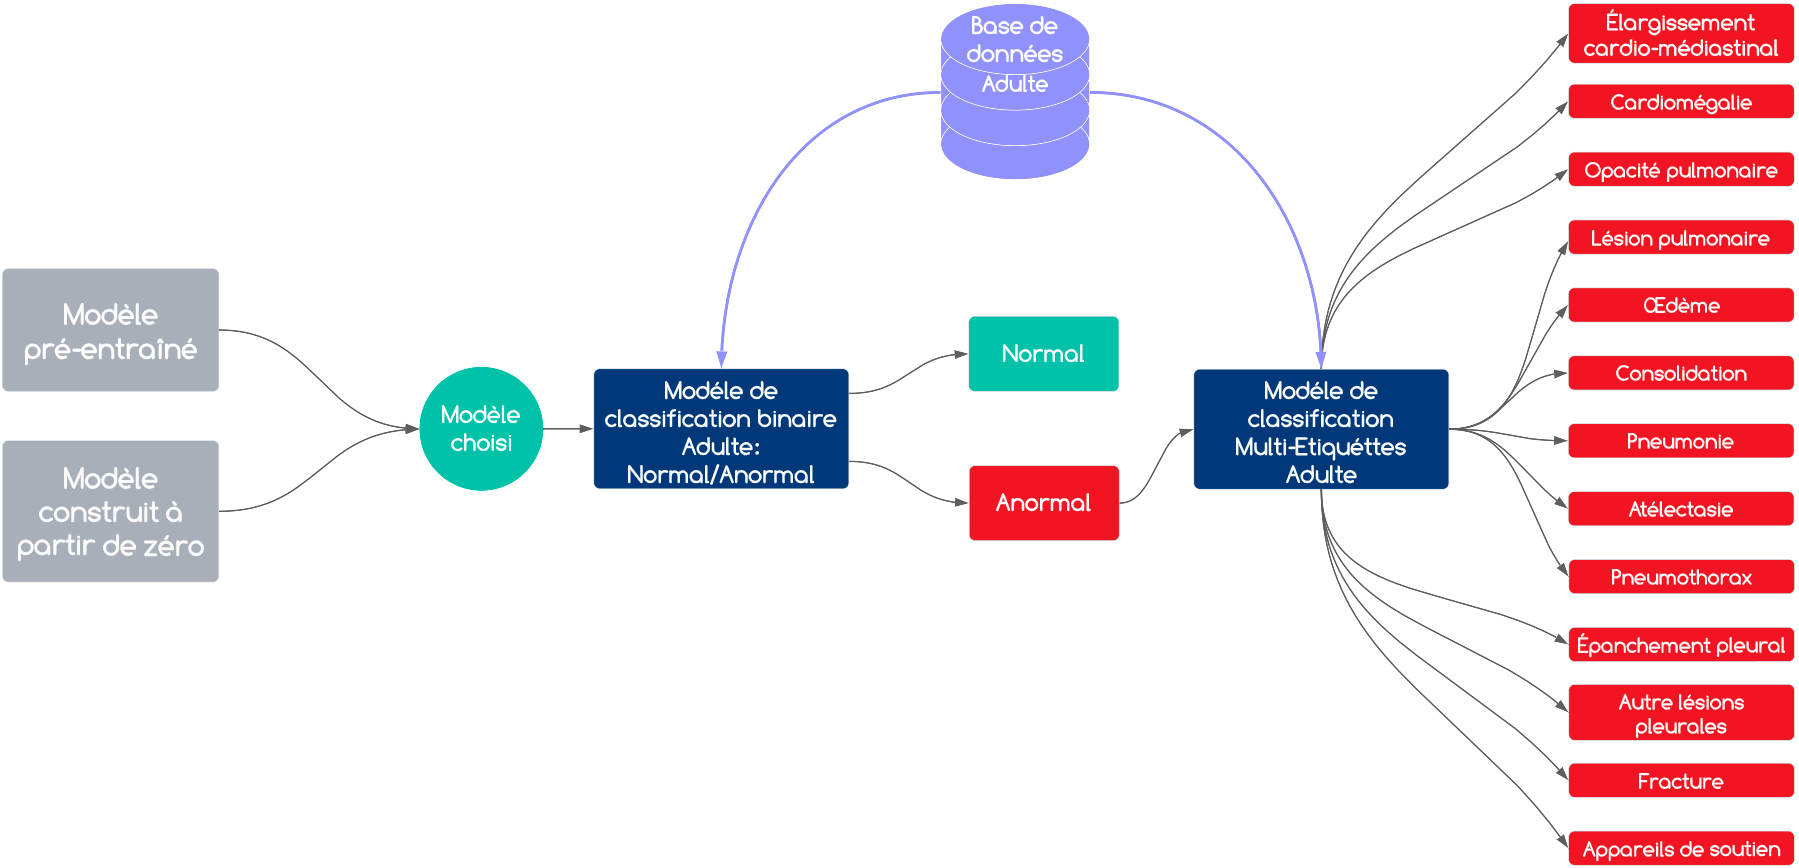
\includegraphics[width=1\textwidth]{adulte_model_train.png}
        \caption{La schéma de créeation du modèle des radiographies adultes}\label{fig:adulte_model_schema}
    \end{figure}
    \begin{figure}[H]
        \centering
        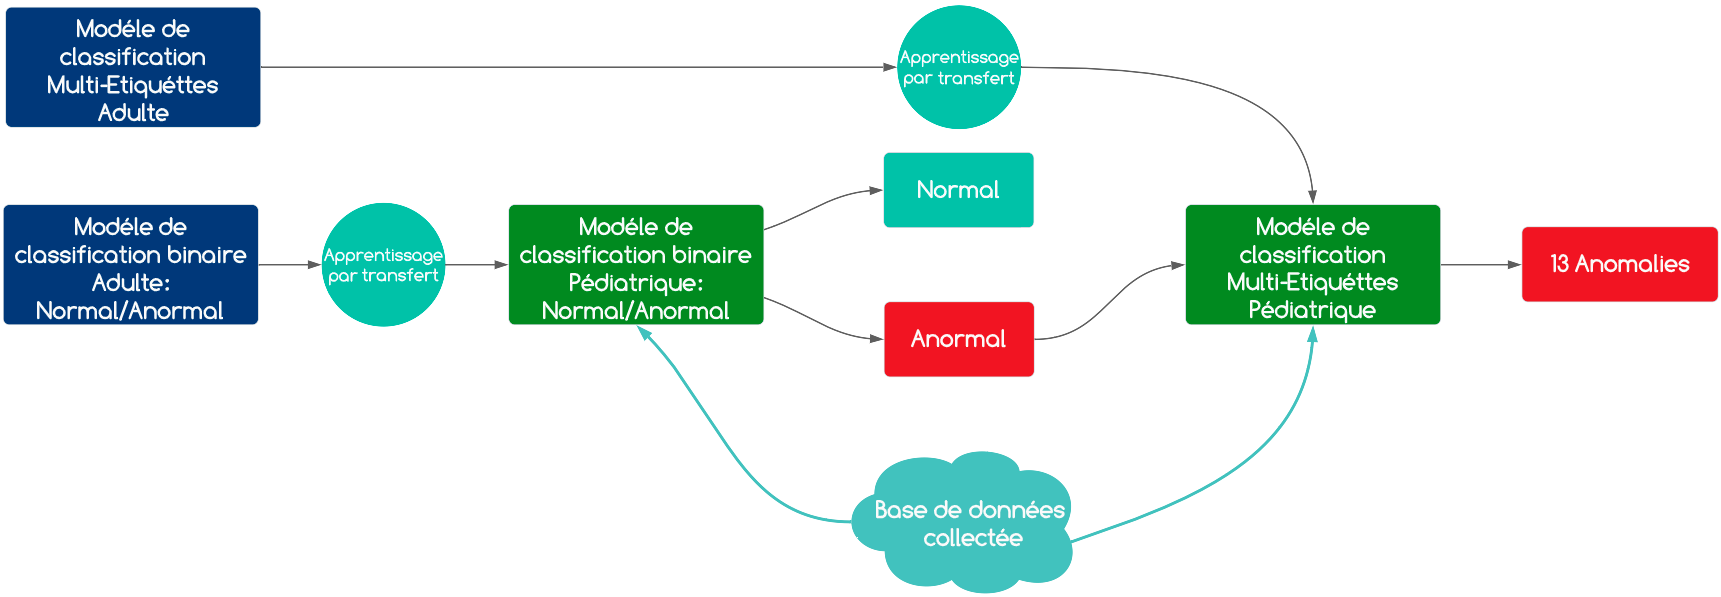
\includegraphics[width=1\textwidth]{pedia_model_train.png}
        \caption{La schéma de créeation du modèle des radiographies adultes}\label{fig:pedia_model_schema}
    \end{figure}
\section{Choix techniques}
Cette partie est consacrée à la présentation de l'environnement matériel et logiciel utilisé pour développer la solution proposée. Expliquer les décisions techniques concernant les langages de programmation et les outils à utiliser.
    \subsection{Architecture logicielle}
    \subsection{API}
    API signifie Application Programming Interface. En termes simples, une API est un ensemble de fonctions et de procédures qui vous permettent de créer une application. Accéder aux données et fonctionnalités d'autres applications, services ou systèmes d'exploitation. 
    Vous êtes essentiellement un intermédiaire entre différentes plates-formes logicielles. Ils permettent à deux applications indépendantes de "parler" entre elles. 
    Par exemple, supposons que vous êtes un agent de change fortement impliqué dans les marchés financiers et le trading. L'API peut lier un ensemble d'algorithmes de trading automatisés à la plateforme de courtage de trading préférée d'un trader. Il permet aux traders de visualiser les cotations et les données de prix en temps réel, ainsi que d'effectuer des transactions électroniques.

    \begin{figure}[H]
        \centering
        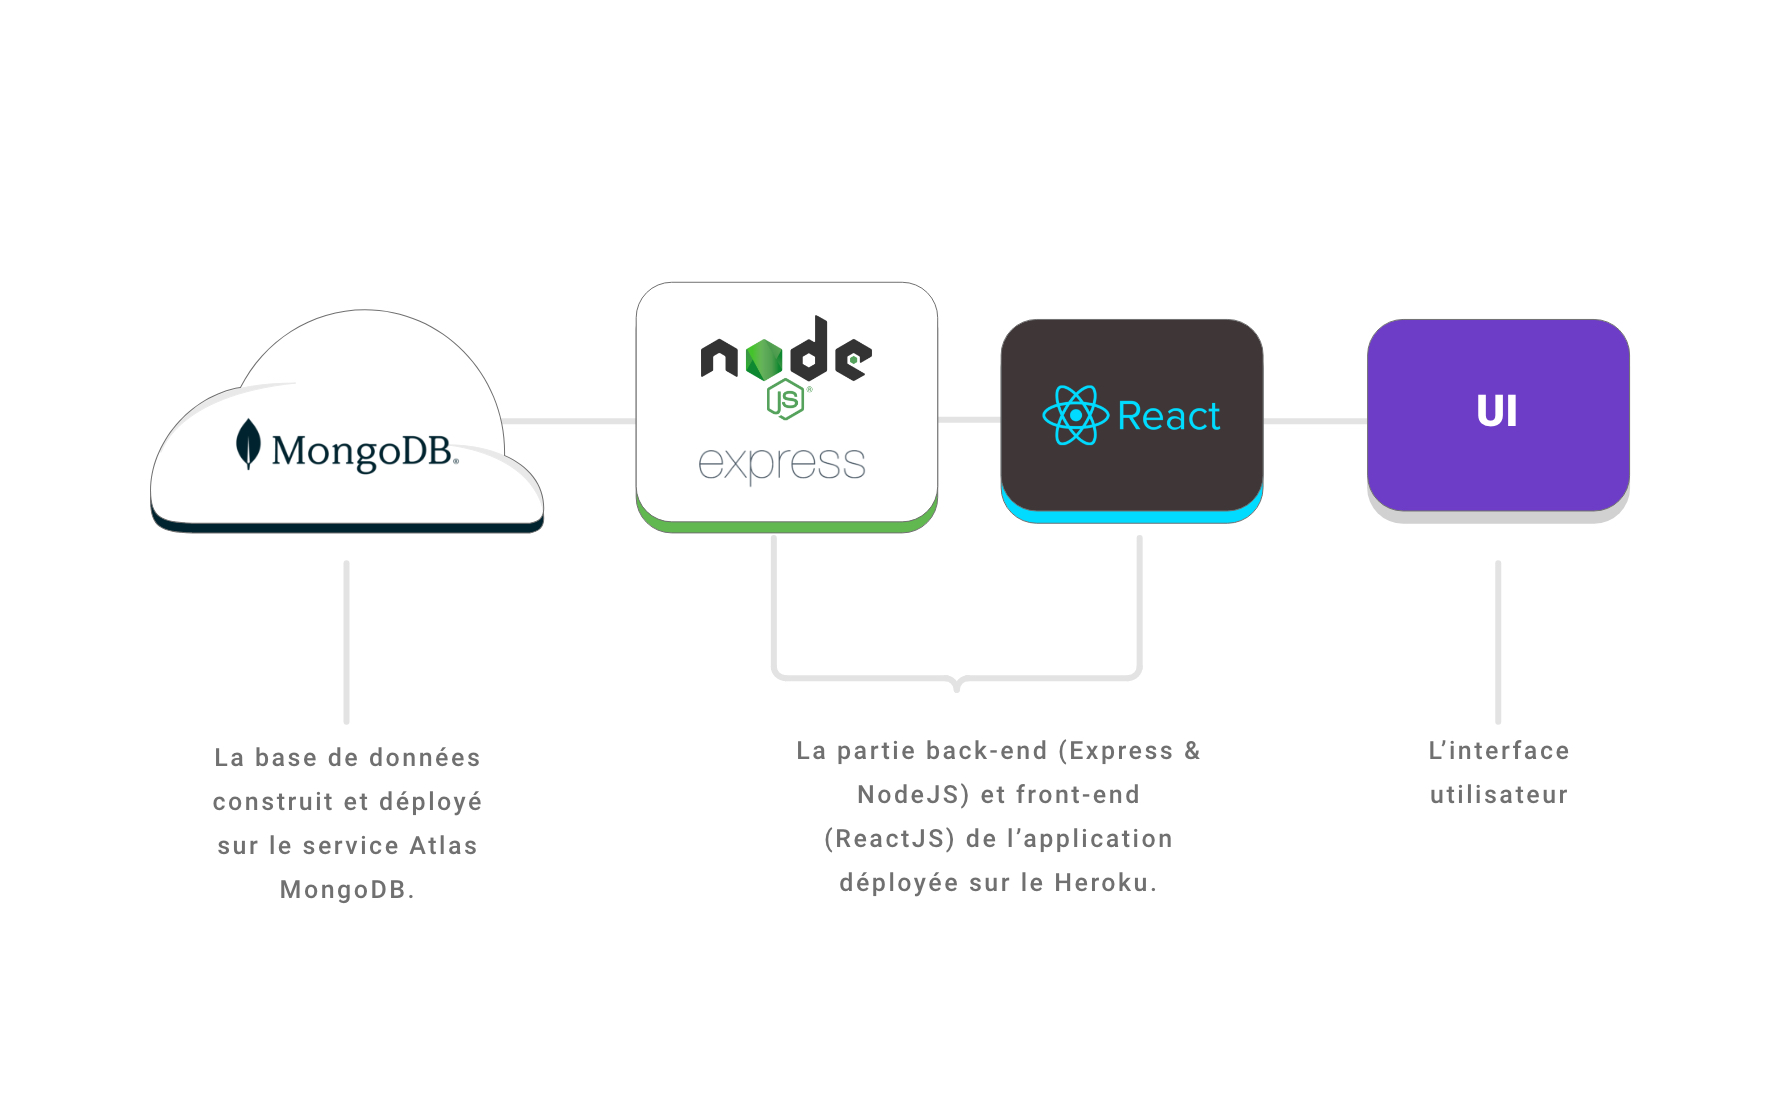
\includegraphics[width=1\textwidth]{log_arc.jpg}
        \caption{La schéma de logicielle de l'application web Xpedia}\label{fig:log_arc}
    \end{figure}

    \subsubsection{MERN stack}
    \begin{figure}[H]
        \centering
        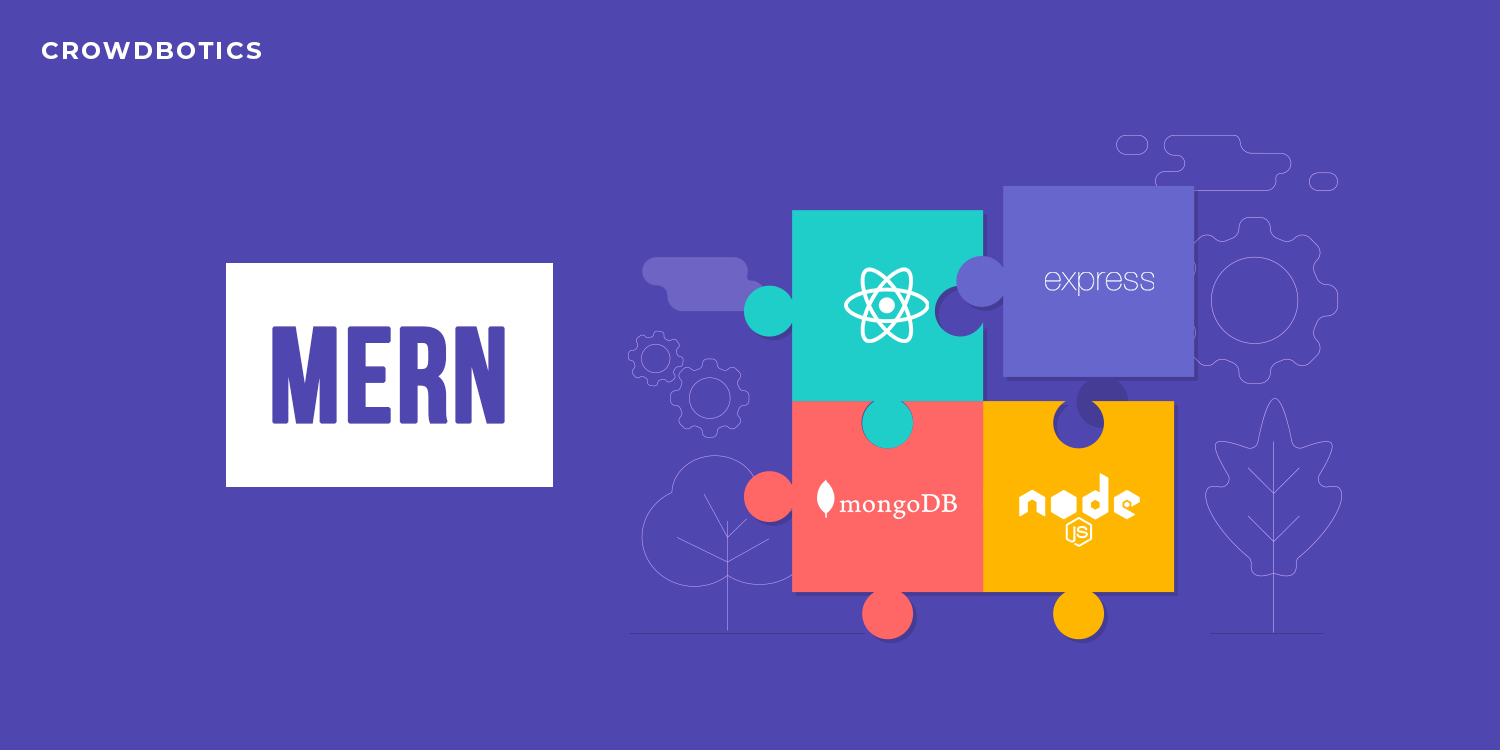
\includegraphics[width=0.6\textwidth, trim={5cm, 3cm, 5cm, 5cm},clip]{MERN.png}
        \caption{Le logo du MERN stack}\label{fig:mern}
    \end{figure}
    \paragraph{MERN Stack} est un ensemble de technologies puissantes et fiables utilisées pour développer des applications informatiques évolutives qui incluent des composants back-end, front-end et de base de données. JavaScript est utilisé pour développer des sites Web entiers plus rapidement et plus facilement.

    C'est une technologie qui est un framework JavaScript complet et convivial pour la création d'applications et de sites Web dynamiques.

    \paragraph{Pour quoi MERN?}MERN stack séparé en deux composants: le back-end et le front-end. De plus, l'ensemble du système de base de données est isolé du reste.

    L'ensemble du système, y compris le front-end, le back-end et la base de données, utilise l'API REST, qui agit comme un "middleware" et est réutilisable pour toute autre application: logiciel mobile, etc., très facilement.

    L'API REST vous permet de connecter des applications entre elles comme les pièces d'un puzzle. Les API REST sont basées sur HTTP et imitent les styles de communication Web, ce qui les rend très avantageuses à utiliser dans MERN.
    \begin{enumerate}\bfseries
        \item Atlas MongoDB\newline
        \begin{figure}[H]
            \centering
            
\includegraphics[width=0.6\textwidth]{atlass_mdb.png}
            \caption{Logo de Atlas MongoDB}\label{fig:atlass_mdb}
        \end{figure}
        \normalfont
        MongoDB Atlas est une plateforme de données de développeur multi-cloud. Au cœur se trouve notre base de données cloud entièrement gérée pour les applications modernes. Atlas est le meilleur moyen d'exécuter MongoDB, la principale base de données non relationnelle. Le modèle de document de MongoDB est le moyen le plus rapide d'innover car les documents correspondent directement aux objets de votre code. En conséquence, ils sont beaucoup plus faciles et plus naturels à travailler. Vous pouvez stocker des données de n'importe quelle structure et modifier votre schéma à tout moment lorsque vous ajoutez de nouvelles fonctionnalités à vos applications.

        Atlas Database est disponible dans plus de 80 régions sur AWS, Google Cloud et Azure. Vous pouvez même tirer parti des déploiements multi-cloud et multi-régions, ce qui vous permet de cibler les fournisseurs et les régions qui servent le mieux vos utilisateurs. Une automatisation de pointe et des pratiques éprouvées garantissent la disponibilité, l'évolutivité et la conformité aux normes de sécurité et de confidentialité des données les plus exigeantes.
        \bfseries
        \item Express Node js\newline
        \begin{figure}[H]
            \centering
            
\includegraphics[width=0.6\textwidth]{react.png}
            \caption{Logo de ReactJS}\label{fig:react}
        \end{figure}
        \normalfont
        Express est un cadre d'application Web Node.js minimal et flexible qui fournit un ensemble  de fonctionnalités robustes pour les applications Web et mobiles. 
        Express fournit une fine couche de fonctionnalités d'application Web de base sans masquer les fonctionnalités familières de Node.js.
        \bfseries
        \item React\newline
        \begin{figure}[H]
            \centering
            
\includegraphics[width=0.6\textwidth]{react.png}
            \caption{Logo de ReactJS}\label{fig:react}
        \end{figure}
        \normalfont
        React est une bibliothèque JavaScript pour créer des interfaces utilisateur. 

        Déclaratif: React facilite la création d'interfaces utilisateur interactives. Concevez une vue simple pour chaque état de votre application et React mettra à jour et affichera efficacement le composant approprié à mesure que les  données changent. Une vue déclarative rend votre code plus prévisible, plus facile à comprendre et plus facile à déboguer. 
 
        Basé sur les composants: créez des composants encapsulés qui gèrent leur propre état et combinez-les pour créer des interfaces utilisateur complexes. Étant donné que la logique des composants est écrite en JavaScript au lieu de modèles, vous pouvez facilement transmettre de grandes quantités de données  via votre application et conserver l'état en dehors du DOM.
 
        Apprenez une fois, écrivez n'importe où: nous ne faisons aucune hypothèse sur le reste de la pile technologique, vous pouvez donc développer de nouvelles fonctionnalités dans React sans réécrire le code existant. React peut également utiliser Node pour le rendu sur le serveur  et React Native pour exécuter des applications mobiles.

        \bfseries
    \end{enumerate}
    \subsubsection{Heroku}
    \begin{figure}[H]
        \centering
        
\includegraphics[width=0.6\textwidth]{heroku.png}
        \caption{Logo de Heroku}\label{fig:heroku}
    \end{figure}

    Heroku est une plate-forme de services cloud qui a gagné en popularité  ces dernières années. Heroku est si facile à utiliser qu'il est devenu le choix incontournable pour de nombreux projets de développement. 
    L'accent mis sur la prise en charge des applications centrées sur le client facilite le développement et le déploiement  des applications. Les entreprises utilisant Heroku peuvent se concentrer sur le perfectionnement de leurs applications, tandis que la plateforme Heroku gère le matériel et les serveurs. Ce n'est pas l'infrastructure qui les soutient.

    \subsubsection{Visual Studio Code}
    \begin{figure}[H]
        \centering
        
\includegraphics[width=0.6\textwidth]{vscode.png}
        \caption{Logo de Visual Studio Code}\label{fig:vscode}
    \end{figure}
    Visual Studio Code est un éditeur de code source léger mais puissant qui s'exécute sur votre bureau et est disponible sur Windows, macOS et Linux. Il offre un support intégré pour JavaScript, TypeScript et Node.js, et dispose d'un riche écosystème d'extensions pour d'autres langages et runtimes (C, C\#, Java, Python, PHP, Go, dotNET, etc.).

    Visual Studio Code combine la simplicité d'un éditeur de code source avec de puissants outils de développement comme la complétion et le débogage de code IntelliSense. 
 C'est avant tout un éditeur qui plie. Le cycle édition-construction-débogage est si fluide que vous passez moins de temps à vous occuper des environnements et plus de temps à concrétiser vos idées.

    \subsection{Outils d'apprentissage automatique et de préparation des données}
    \subsubsection{Python}
    \begin{figure}[H]
        \centering
        
\includegraphics[width=0.6\textwidth]{python.png}
        \caption{Logo de Python}\label{fig:python}
    \end{figure}

    Python est un langage de programmation polyvalent populaire qui peut être utilisé pour une grande variété d'applications. Il comprend des structures de données de haut niveau, un typage dynamique, une liaison dynamique et de nombreuses autres fonctionnalités qui aident à développer des applications aussi  complexes que  le "code de colle" qui relie les scripts et les composants. Vous pouvez également  effectuer des appels système pour presque tous les systèmes d'exploitation et les étendre pour exécuter du C ou du code écrit en C. En raison de son omniprésence et de sa capacité à s'exécuter sur presque toutes les architectures système, Python est un langage universel qui peut être utilisé dans une grande variété d'applications.

    \subsubsection{Librairies}
    La bibliothèque standard de Python est très étendue et offre un large éventail de fonctionnalités. Cette bibliothèque contient des modules intégrés (écrits en C) qui permettent d'accéder à des fonctionnalités  système telles que les E/S de fichiers qui sont inaccessibles aux programmeurs Python, et des modules  Python qui fournissent des solutions standardisées à de nombreux problèmes quotidiens. programmation. Certains de ces modules sont explicitement conçus pour faciliter et améliorer la portabilité des programmes Python en faisant abstraction des spécificités de la plate-forme dans des API indépendantes de la plate-forme.
    \begin{enumerate}\bfseries
        \item Numpy
        \begin{figure}[H]
            \centering
            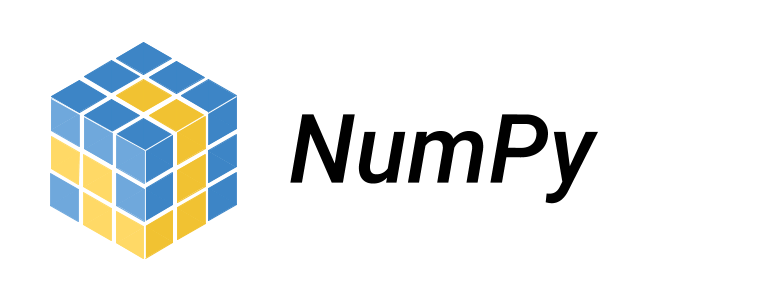
\includegraphics[width=0.6\textwidth]{numpy.png}
            \caption{Logo de Numpy}\label{fig:numpy}
        \end{figure}
        \normalfont
        NumPy est un package de traitement de tableau à usage général. Fournit des objets et des outils de tableau multidimensionnel hautes performances  pour manipuler ces tableaux. Package de base pour le calcul scientifique  Python. C'est un logiciel open source.Il contient diverses fonctionnalités dont ces importantes:
        \begin{itemize}[label=$\bullet$]
            \item Puissants objets de tableaux N-dimensionnels 
            \item Fonctions sophistiquées (diffusion)
            \item Outils d'intégration de code C/C et Fortran
            \item Compétences utiles en algèbre linéaire, transformées de Fourier et nombres aléatoires
        \end{itemize}  
        
        En plus de ses utilisations scientifiques évidentes, NumPy est un outil efficace Il peut également être utilisé comme  conteneur de données  multidimensionnel à usage général. Vous pouvez définir n'importe quel type de données  à l'aide de Numpy. Cela signifie que NumPy peut être intégré de manière transparente et rapide dans de nombreuses bases de données.

        \bfseries
        \item Pandas
        \begin{figure}[H]
            \centering
            
\includegraphics[width=0.6\textwidth]{pandas.png}
            \caption{Logo de Pandas}\label{fig:pandas}
        \end{figure}
        \normalfont
        Pandas est l'un des outils de science des données et d'apprentissage automatique les plus utilisés pour nettoyer et analyser les données. 
        Pandas est l'outil de choix pour traiter ces données désordonnées du monde réel.  pandas est l'un des packages Python open source basés sur NumPy. 
        Le traitement des données avec pandas est très rapide et efficace en utilisant des séries et des dataframes pandas. Ces deux structures de données pandas sont utiles pour manipuler les données de différentes manières. 
        En ce basant sur les fonctionnalités disponibles dans  pandas, nous pouvons dire que  pandas est le mieux adapté au traitement des données. Il peut gérer les données manquantes, nettoyer les données et prendre en charge plusieurs formats de fichiers. Cela signifie que vous pouvez lire et charger des données dans de nombreux formats tels que CSV, Excel, SQL, etc.


        \bfseries
        \item OpenCV
        \begin{figure}[H]
            \centering
            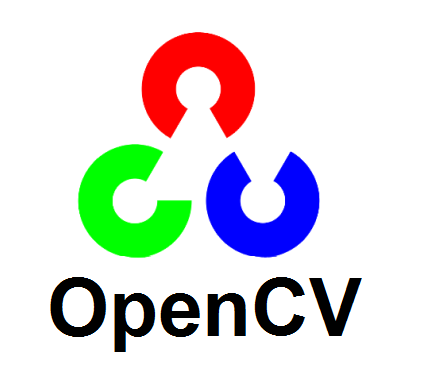
\includegraphics[width=0.6\textwidth]{opencv.png}
            \caption{Logo de Open Computer Vision}\label{fig:opencv}
        \end{figure}
        \normalfont
        OpenCV (Open Source Computer Vision Library) est une bibliothèque de logiciels open source de vision par ordinateur et d'apprentissage automatique. OpenCV a été développé pour fournir une infrastructure commune pour les applications de vision par ordinateur et  accélérer l'utilisation de la vision artificielle dans les produits commerciaux. OpenCV est un produit sous licence BSD, les entreprises peuvent donc facilement utiliser et  modifier  le code.
        
        La bibliothèque contient plus de 2500 algorithmes optimisés, y compris un ensemble complet d'algorithmes de vision par ordinateur et d'apprentissage automatique classiques et  de pointe. Ces algorithmes sont utilisés pour la détection et la reconnaissance de visages, l'identification d'objets, la classification du comportement humain dans les vidéos, le suivi de mouvement de caméra, le suivi d'objets en mouvement, l'extraction de modèles 3D d'objets, les nuages de points 3D à partir de caméras stéréo, Résolution d'images à travers des scènes, recherche d'images similaires dans des bases de données d'images, suppression des yeux rouges des images prises au flash, suivi des mouvements oculaires, détection de paysages, création de marqueurs à superposer avec la réalité augmentée, etc. OpenCV a une communauté de plus de 7 000 utilisateurs avec plus de 18 millions de téléchargements estimés. Cette bibliothèque est fréquemment utilisée par les entreprises, les groupes de recherche et les agences gouvernementales.

        \bfseries
        \item Tensorflow
        \begin{figure}[H]
            \centering
            
\includegraphics[width=0.6\textwidth]{tensorflow.png}
            \caption{Logo de Tensorflow}\label{fig:tensorflow}
        \end{figure}
        \normalfont
        TensorFlow est une plate-forme d'apprentissage automatique open source de bout en bout. TensorFlow est un système complet de gestion de tous les aspects des systèmes d'apprentissage automatique. Cependant, ce cours se concentre sur le développement et la formation de modèles d'apprentissage automatique à l'aide d'API TensorFlow spécifiques. 
        
        L'API TensorFlow est organisée de manière hiérarchique, avec des API de  niveau supérieur construites au-dessus des API de niveau inférieur. Les chercheurs en apprentissage automatique utilisent des API de bas niveau pour créer et explorer de nouveaux algorithmes d'apprentissage automatique. En utilisant tf.keras on peut définir et former des modèles d'apprentissage automatique  pour effectuer des prédictions. tf.keras est la version TensorFlow de l'API Keras open source.

        \bfseries
        \item Keras
        \begin{figure}[H]
            \centering
            
\includegraphics[width=0.6\textwidth]{keras.png}
            \caption{Logo de Keras}\label{fig:keras}
        \end{figure}
        \normalfont
        Keras est une API d'apprentissage en profondeur de haut niveau développée par Google pour la mise en œuvre de réseaux de neurones. Il est écrit en Python et est utilisé pour faciliter la mise en œuvre de réseaux de neurones. Il prend également en charge plusieurs calculs de  réseaux neuronaux principaux. 
        
        Keras est relativement facile à apprendre et à utiliser car il fournit une interface Python avec un haut niveau d'abstraction tout en offrant de multiples possibilités de backend à des fins de calcul. Cela rend Keras plus lent que les autres frameworks d'apprentissage en profondeur, mais très convivial pour les débutants.

        \bfseries
        \item Matplotlib
        \begin{figure}[H]
            \centering
            
\includegraphics[width=0.6\textwidth]{matplotlib.jpeg}
            \caption{Logo de Matplotlib}\label{fig:matplotlib}
        \end{figure}
        \normalfont
        Matplotlib est également l'une des bibliothèques les plus réussies et les plus utilisées, fournissant divers outils de visualisation de données en Python. 
        C'est l'une des bibliothèques de traçage les plus puissantes de Python. Il s'agit d'une bibliothèque multiplateforme qui fournit divers outils pour créer des tracés 2D à partir de données de liste ou de tableau en Python. 
        
        Matplotlib a été créé en 2003 dans le langage de programmation Python par Jean D. Hunter. Il utilise NumPy, une bibliothèque qui fournit des extensions mathématiques numériques pour Python. 
        
        Il expose également une API orientée objet qui vous permet d'étendre la possibilité de placer des graphiques statiques dans votre application à l'aide de divers kits d'outils d'interface graphique Python disponibles (Tkinter, PyQt, etc.). 
        Vous pouvez utiliser différents types de graphiques pour visualiser vos données et faciliter leur compréhension. En écrivant quelques lignes de code en Python, vous pouvez utiliser ces différents types de graphiques (scatter plots, histograms, bar charts, error charts, box charts, etc.).

        \bfseries
    \end{enumerate}
    \subsubsection{IDEs}
    \begin{enumerate}\bfseries
        \item Jupyter
        \begin{figure}[H]
            \centering
            
\includegraphics[width=0.6\textwidth]{jupyter.jpeg}
            \caption{Logo de Jupyter}\label{fig:jupyter}
        \end{figure}
        \normalfont
        Jupyter est une application Web permettant de programmer dans plus de 40 langages de programmation, dont Python, Julia, Ruby, R ou  Scala. Il s'agit d'un projet communautaire visant à développer des logiciels libres, des formats ouverts et des services pour l'informatique interactive. Jupyter est une évolution du projet IPython. Jupyter vous permet de créer des blocs-notes, des programmes contenant à la fois du texte  et du code Markdown. Ces cahiers sont utilisés  pour explorer et analyser des données en science des données.

        \bfseries
        \item Google Colab pro+
        \begin{figure}[H]
            \centering
            
\includegraphics[width=0.6\textwidth]{colab.png}
            \caption{Logo de Colab}\label{fig:colab}
        \end{figure}
        \normalfont
        Le service Google Colaboratory, ou Google Colab en abrégé, vous permet d'exécuter du code Python dans un navigateur Web dans ce que l'on appelle des "notebooks". Il est utilisé pour l'apprentissage en profondeur, le partage et le travail sur des projets de science des données avec d'autres.
        \begin{itemize}[label=$\bullet$]
            \item Cartes graphiques plus rapides
            
            Avec le Colab Pro/Pr, vous pouvez accéder à plus de ressources et  choisir des GPU plus rapides tels que NVIDIA Tesla T
            et NVIDIA Tesla P100 pour vos projets. En tant qu'utilisateur gratuit de Google Colab, je constate souvent que ma carte graphique ralentit et que ma RAM est faible. Lors de la création d'images ki (ki-générated images), le temps de traitement d'image des modèles Pro et Pro est environ 6 fois plus rapide que  le Colab gratuit. De quoi réserver au moins la version Colab Pro pour environ 10 euros par mois. 
            \item Durée d'exécution plus longue 
            
            La version Pro de Google Colab a également une durée d'exécution plus longue, gardant votre ordinateur portable connecté jusqu'à 24 heures, tandis que la version gratuite se déconnecte après seulement 12 heures. 
            L'avantage de la version Colab Pro ici est que l'instance continuera à s'exécuter  après la fermeture de la fenêtre du navigateur, mais dans les versions Free et Pro, la fermeture de la fenêtre mettra fin à l'instance. 
            \item Plus de RAM
            
            Les utilisateurs du modèle payant bénéficient également de plus de RAM. Vous devriez être satisfait de 16 Go pour le Colab gratuit, mais les utilisateurs Pro ont 32 Go et les utilisateurs Pro ont  52 Go de RAM. Les comptes payants sont particulièrement adaptés au traitement de grandes quantités de données.
        \end{itemize}
        
       
        \bfseries
    \end{enumerate}
    \subsubsection{HPC-MARWAN}
    \begin{figure}[H]
        \centering
        
\includegraphics[width=0.6\textwidth]{marwan-hpc.png}
        \caption{Logo de HPC-MARWAN}\label{fig:marwan-hpc}
    \end{figure}
    Le Centre National de la Recherche Scientifique et Technique met à la disposition de la communauté des chercheurs marocains une infrastructure de Calcul Haute Performance (HPC) accessible à distance.

    L'infrastructure compte 38 nœuds avec la capacité suivante:
    • 1672 cœurs de processeur (165 TFlops)
    • 396 To de stockage
    • 10,4 To de RAM
    • 4 GPU

    Les nœuds sont interconnectés via un réseau à faible latence à une bande passante de 100 Gbps, optimisant ainsi les performances de calcul parallèle. Un système de fichiers parallèle est implémenté pour faciliter un accès haute performance via des IOPS simultanées par plusieurs tâches d'une application parallèle.
    L'infrastructure est connectée à MARWAN via une liaison 5Gbps pour assurer des vitesses de transfert de données élevées depuis les universités et institutions connectées à MARWAN.

    \subsubsection*{SLURM Workload Manager}
    SLURM: Simple Linux Utility for Resource Management
    \begin{figure}[H]
        \centering
        
\includegraphics[width=0.6\textwidth]{slurm.png}
        \caption{Logo de SLURM}\label{fig:slurm}
    \end{figure}

    Slurm est un système de gestion de cluster et de planification des tâches open source, tolérant aux pannes et hautement évolutif pour les grands et petits clusters Linux. Slurm ne nécessite aucune modification du noyau pour son fonctionnement et est relativement autonome. En tant que gestionnaire de charge de travail de cluster, Slurm a trois fonctions clés. Premièrement, il alloue un accès exclusif et/ou non exclusif aux ressources (noeuds de calcul) aux utilisateurs pendant une certaine durée afin qu'ils puissent effectuer un travail. Deuxièmement, il fournit un cadre pour démarrer, exécuter et surveiller le travail (normalement un travail parallèle) sur l'ensemble des noeuds alloués. Enfin, il arbitre les conflits de ressources en gérant une file d'attente de travaux en attente. Des plug-ins facultatifs peuvent être utilisés pour la comptabilité, la réservation avancée, la planification des équipes (partage du temps pour les tâches parallèles), la planification des remplissages, la sélection des ressources optimisée pour la topologie, les limites de ressources par utilisateur ou compte bancaire et les algorithmes sophistiqués de hiérarchisation des tâches multifactorielles.

\section{Bases de données}
    Durant notre recherche pour une base de données convenable a notre projet on a trouver la liste des bases de données suivnates :
    \begin{table}[H]
        \centering
        \scriptsize
        \begin{tabularx}{\textwidth}{ |X|X|X|X|X|X|X|X| } 
            \hline
            \hfil Nom de base de données & \hfil Nombre des images & \hfil Pourcentage des images pédiatriques & \hfil Tranche d'âge & \hfil Étiquettes de recherche et de diagnostic & Étiquettes 
            \hfil spatiales & \hfil Taille de l'image & \hfil Statut d'accès\\ [1ex]
            \hline
            \hfil ChestX-Ray14 & \hfil 112120 & \hfil - & \hfil - & \hfil 14 & \hfil 0 & \hfil redimensionné 1024 x 1024 & \hfil - \\ 
            \hline
            \hfil PLCO & \hfil 185421 & \hfil - & \hfil - & \hfil 12 & \hfil 9 & \hfil taille originale & \hfil - \\ 
            \hline
            \hfil CheXpert & \hfil 224316 & \hfil 0\% & \hfil 18+ & \hfil 14 & \hfil 0 & \hfil taille originale & \hfil public \\ 
            \hline
            \hfil MIMIC-CXR & \hfil 371920 & \hfil - & \hfil - & \hfil 14 & \hfil 0 & \hfil taille originale & \hfil - \\ 
            \hline
            \hfil PadChest & \hfil 160868 & \hfil 34\% & \hfil - & \hfil 193 & \hfil 104 & \hfil taille originale & \hfil public \\
            \hline
            \hfil Kermany & \hfil 5856 & \hfil 100\% & \hfil 1-5 & \hfil 3 & \hfil 0 & \hfil taille originale & \hfil - \\ 
            \hline
            \hfil PERCH & \hfil 3587 & \hfil - & \hfil - & \hfil 5 & \hfil - & \hfil - & \hfil - \\
            \hline
            \hfil NIH-14 & \hfil 112120 & \hfil 46\% & \hfil 1–17 & \hfil 14 & \hfil 8 & \hfil 1024 x 1024 & \hfil - \\
            \hline
            \hfil RSNA & \hfil 30227 & \hfil 65\% & \hfil 1–17 & \hfil 3 & \hfil - & \hfil 1024 x 1024 & \hfil - \\
            \hline
            \hfil SIIM – ACR & \hfil 12047 & \hfil 19,53\% & \hfil 1–17 & \hfil 2 & \hfil - & \hfil 1024 x 1024 & \hfil - \\
            \hline
            \hfil NIAID & \hfil 6251 & \hfil 11\% & \hfil 1–17 & \hfil - & \hfil - & \hfil - & \hfil - \\
            \hline
            \hfil Shenzhen & \hfil 662 & \hfil 4,6\% & \hfil 2 mois - 17 anns & \hfil - & \hfil - & \hfil taille originale & \hfil - \\
            \hline
            \hfil Montgomery County & \hfil 138 & \hfil 12,3\% &  \hfil 4–17 & \hfil - & \hfil - & \hfil taille originale & \hfil - \\
            \hline
        \end{tabularx}
        \caption{Les bases données taitants le même phénomène}\label{table:all_dbs}
    \end{table}
    \subsection{CheXpertDB}\label{chexpertDB}
    Le choix de cette  jeu de données de CheXpert comme base du modèle de pré-entraînement est justifié devant :
    \begin{itemize}[label=$\bullet$]
        \item Sa grande taille  ( plus de 224,316  images recueillis rétrospectivement de l'hôpital de Stanford de 65,240 patients. ) 
        \item Son accessibilité au public sans aucune formation préalablement requise
        \item Le nombre important d’anomalies ciblées par l'étiquetage (14) avec une terminologie claire conforme au Glossaire des termes d'imagerie thoracique recommandé par ‘Fleischner Society’ de radiologie thoracique 
        \item l’existence de plusieurs applications sur un sous-ensemble ou  la totalité de ses données via des compétitions avec de haute performances publiées sur son site officiel et des scores d'experts auxquels les chercheurs peuvent comparer leurs modèles.
        

    \end{itemize}
    \subsection{XpediaDB}

\section*{Conclusion}
    \chapter{Réalisation}

\section*{Introduction}

\section{Réalisation}
\subsection{Application web}
\begin{figure}[H]
    \centering
    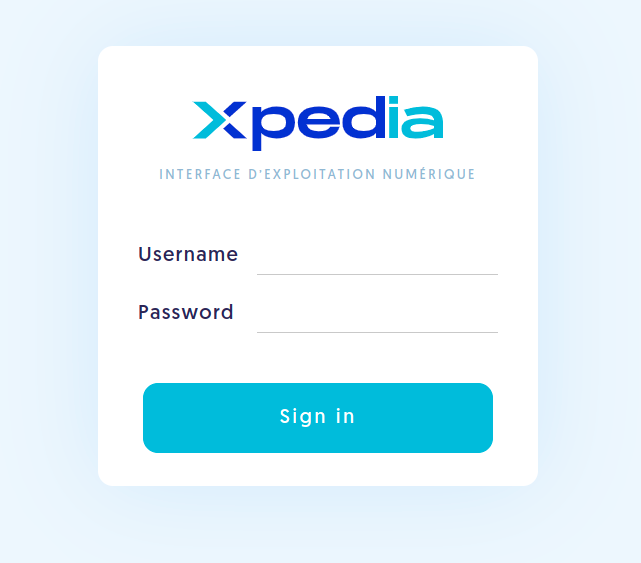
\includegraphics[width=0.8\textwidth]{xpedia_log.png}
    \caption{La login de Xpedia}\label{fig:xpedia_log}
\end{figure}
\begin{figure}[H]
    \centering
    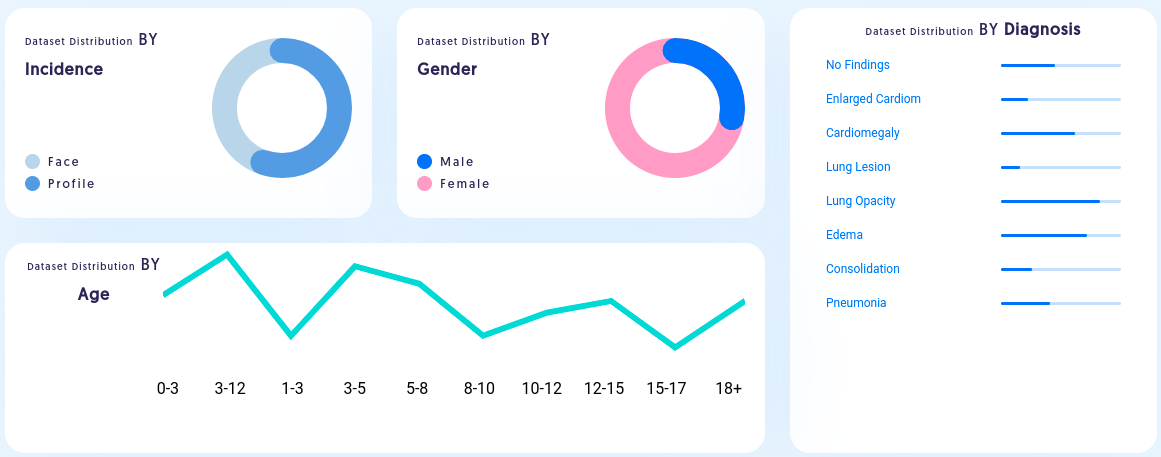
\includegraphics[width=0.8\textwidth]{xpedia_dashboard.png}
    \caption{Le dashboard}\label{fig:xpedia_dashboard}
\end{figure}
\begin{figure}[H]
    \centering
    
\includegraphics[width=0.8\textwidth]{xpedia_menu.png}
    \caption{La menu}\label{fig:xpedia_menu}
\end{figure}
\begin{figure}[H]
    \centering
    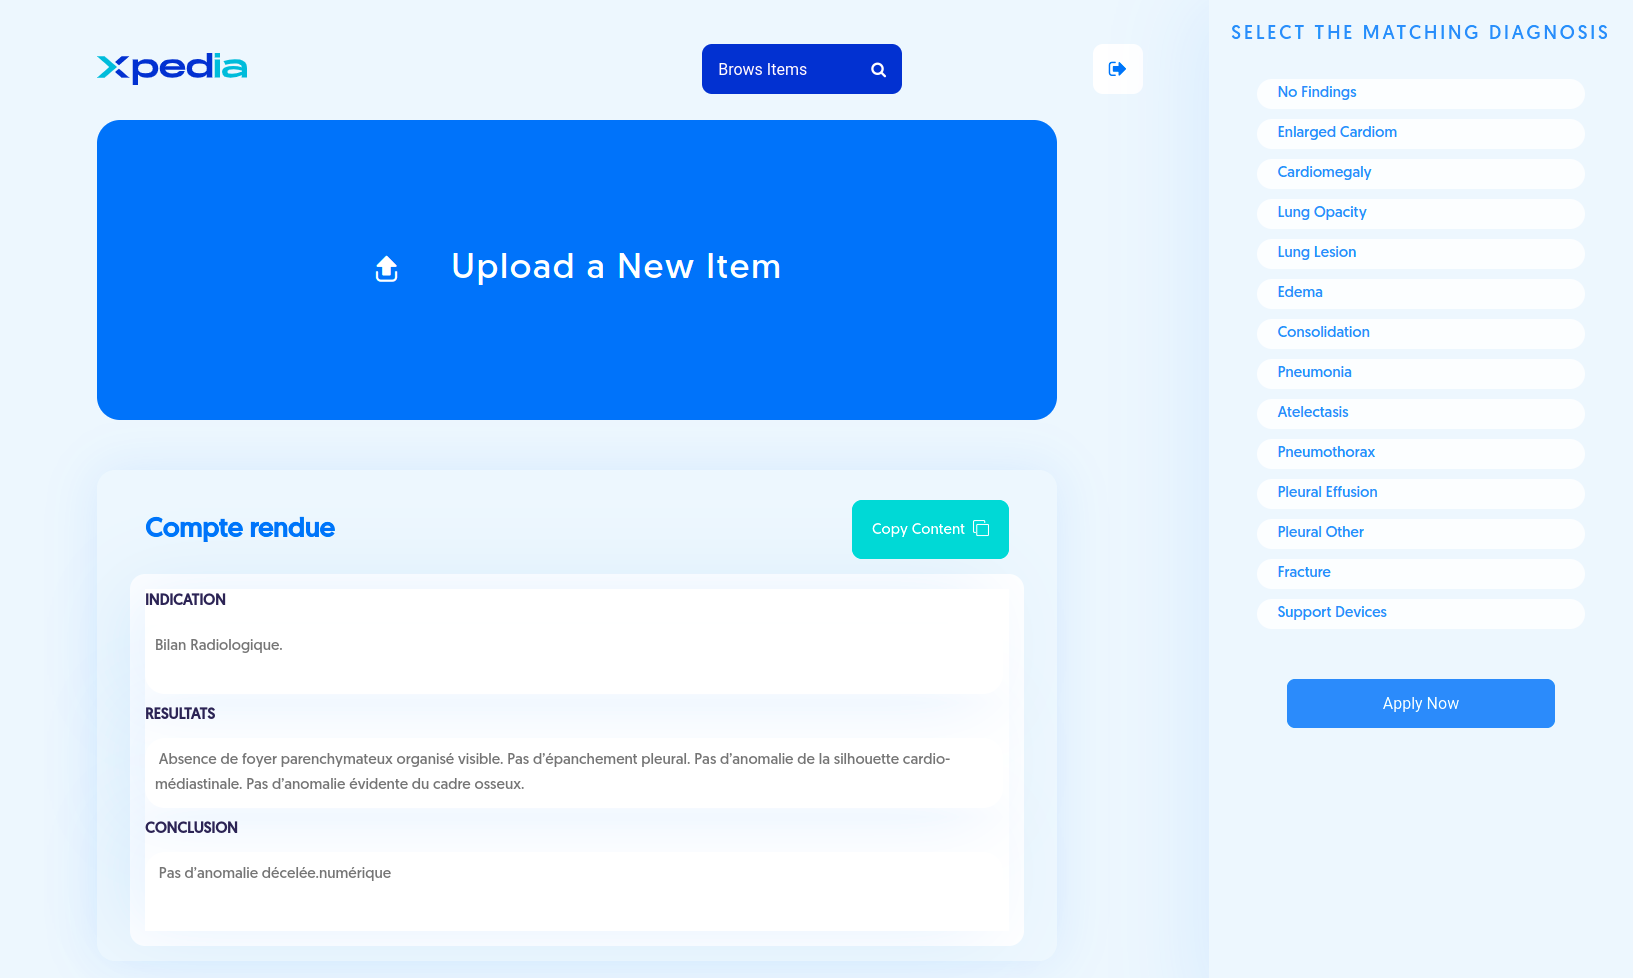
\includegraphics[width=0.8\textwidth]{xpedia_additem.png}
    \caption{La page ajouter élément}\label{fig:xpedia_additem}
\end{figure}
\begin{figure}[H]
    \centering
    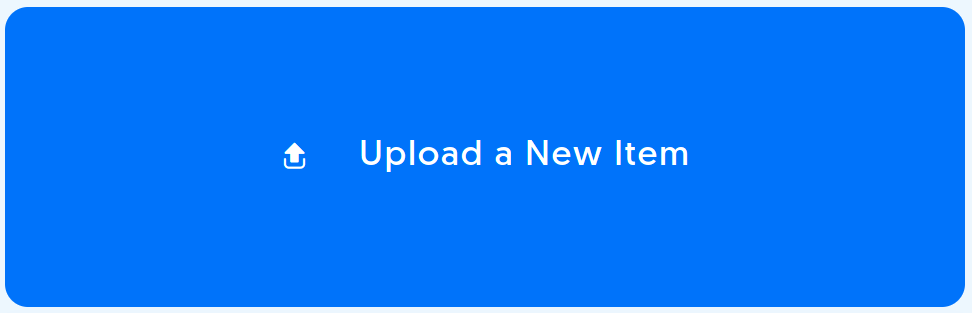
\includegraphics[width=0.8\textwidth]{xpedia_add_image.png}
    \caption{La section réserver à l'ajout d'une image}\label{fig:xpedia_add_image}
\end{figure}
\begin{figure}[H]
    \centering
    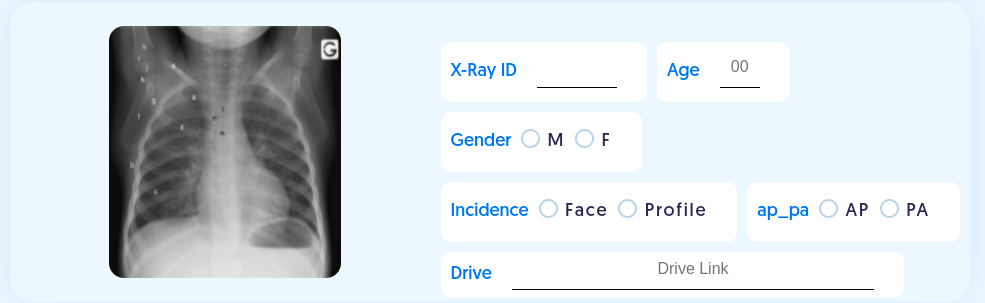
\includegraphics[width=0.8\textwidth]{xpedia_fill_form.png}
    \caption{La formulaire à remplir}\label{fig:xpedia_fill_form}
\end{figure}
\begin{figure}[H]
    \centering
    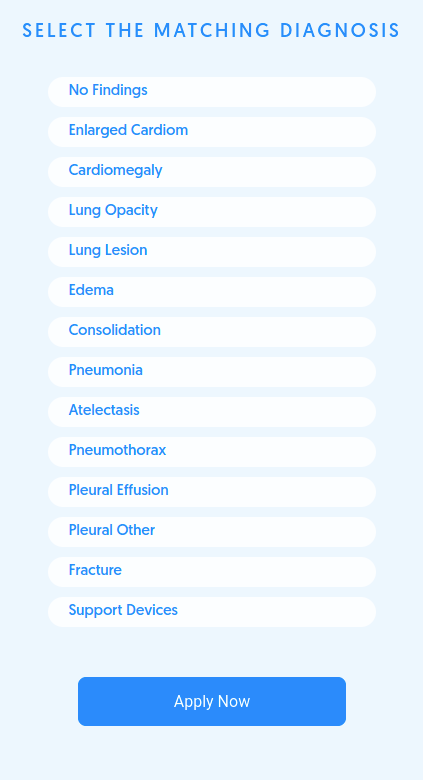
\includegraphics[width=0.8\textwidth]{xpedia_select_section.png}
    \caption{La section de selection des diagnostiques}\label{fig:xpedia_select_section}
\end{figure}
\begin{figure}[H]
    \centering
    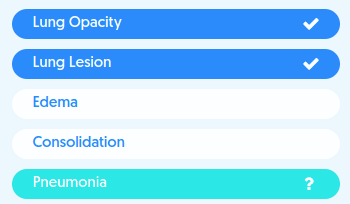
\includegraphics[width=0.8\textwidth]{xpedia_select_items.png}
    \caption{Exemple de selection des diagnostiques}\label{fig:xpedia_select_items}
\end{figure}
\begin{figure}[H]
    \centering
    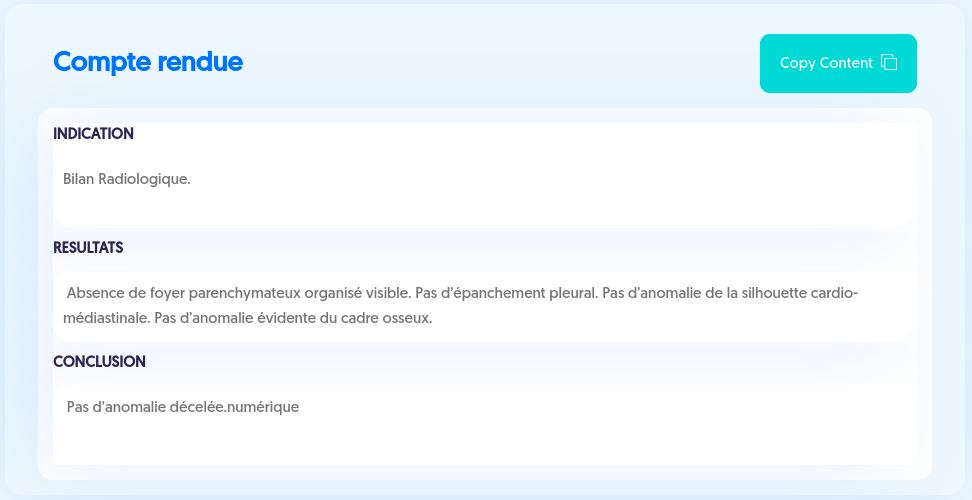
\includegraphics[width=0.8\textwidth]{xpedia_cr}
    \caption{La section du remplissage du compte rendue}\label{fig:xpedia_cr}
\end{figure}
\begin{figure}[H]
    \centering
    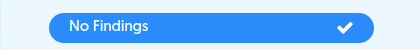
\includegraphics[width=0.8\textwidth]{xpedia_normal_select.png}
    \caption{Choix de 'No Finding' diagnostique}\label{fig:xpedia_menu}
\end{figure}
\begin{figure}[H]
    \centering
    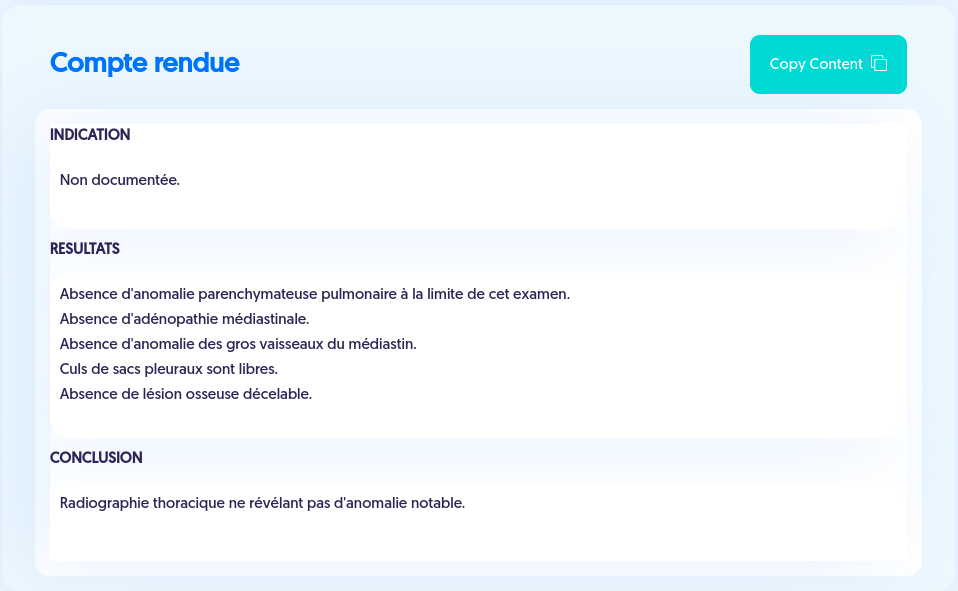
\includegraphics[width=0.8\textwidth]{xpedia_normal_cr.png}
    \caption{Remplissage automatique du compte rendue}\label{fig:xpedia_normal_cr}
\end{figure}
\begin{figure}[H]
    \centering
    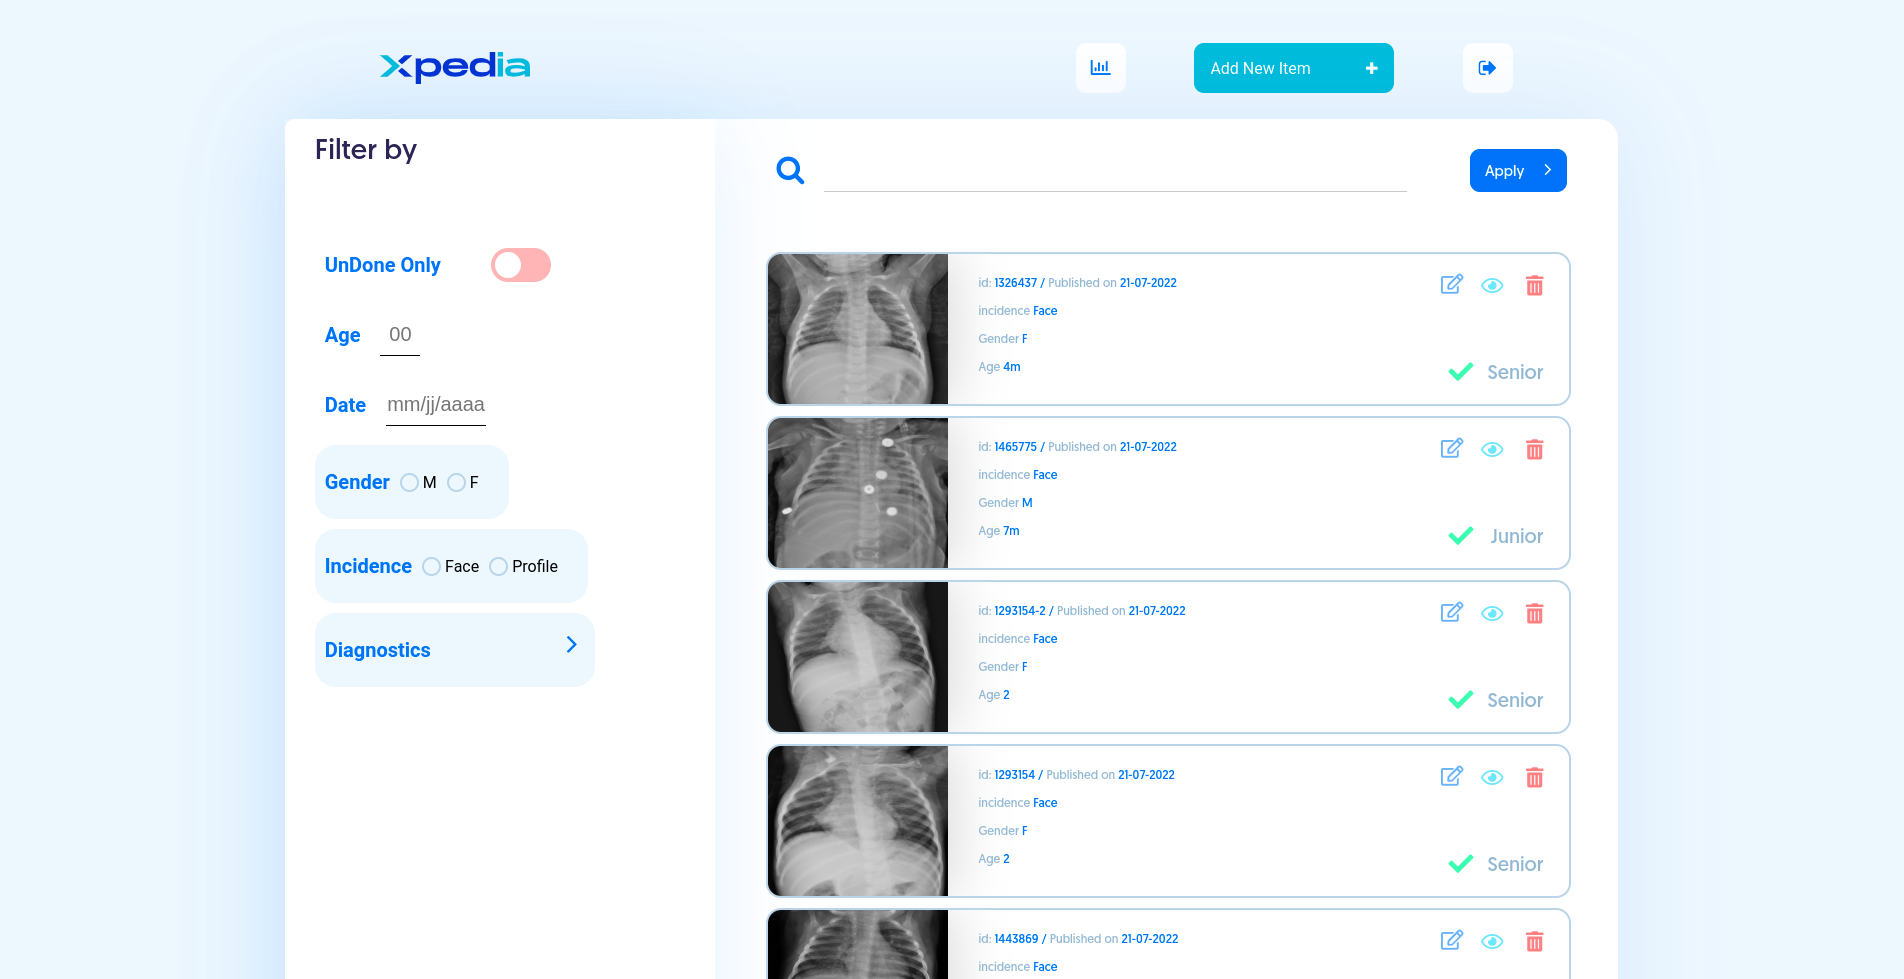
\includegraphics[width=0.8\textwidth]{xpedia_browse_item.png}
    \caption{La page 'browse items'}\label{fig:xpedia_menu}
\end{figure}
\begin{figure}[H]
    \centering
    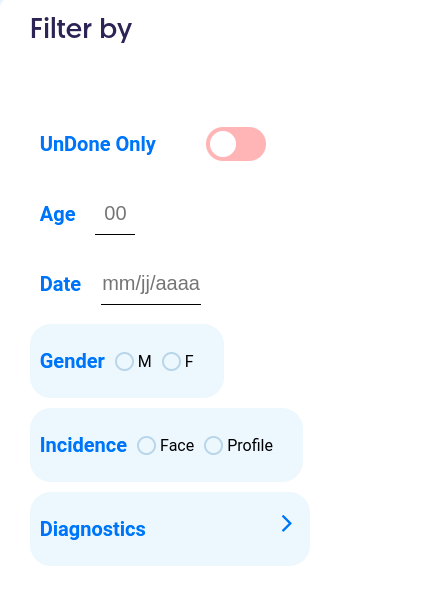
\includegraphics[width=0.8\textwidth]{xpedia_filter_section.png}
    \caption{La section du filtre des éléments}\label{fig:xpedia_filter_section}
\end{figure}
\begin{figure}[H]
    \centering
    \includegraphics[width=0.8\textwidth]{xpedia_research.png}
    \caption{La bar de recherche}\label{fig:xpedia_research}
\end{figure}
\begin{figure}[H]
    \centering
    \includegraphics[width=0.8\textwidth]{xpedia_pagination.png}
    \caption{La menu}\label{fig:xpedia_menu}
\end{figure}
\begin{figure}[H]
    \centering
    \includegraphics[width=0.8\textwidth]{xpedia_item_thumbnail.png}
    \caption{Vignette de l'élément}\label{fig:xpedia_item_thumbnail}
\end{figure}
\begin{figure}[H]
    \centering
    \includegraphics[width=0.8\textwidth]{xpedia_view_page.png}
    \caption{Les détailles de l'élément}\label{fig:xpedia_view_page}
\end{figure}
\begin{figure}[H]
    \centering
    \includegraphics[width=0.8\textwidth]{xpedia_view_showitem.png}
    \caption{Clichés en dimension réel}\label{fig:xpedia_view_showitem}
\end{figure}
\begin{figure}[H]
    \centering
    \includegraphics[width=0.8\textwidth]{xpedia_edit_page.png}
    \caption{La page d'edition de l'élément}\label{fig:xpedia_item_thumbnail}
\end{figure}
\subsection{Preparation des données}
La phase de préparation de données est l'une des phases cruciales dans le projet, le livrable de cette phase est le jeu de données qui alimente le modèle d'apprentissage en profondeur. Pour que ces données soient utiles, elles doivent d'abord être prétraitées selon les étapes déjà décrites dans la section \ref{data_pipeline}. Les figures présentent un exemple de traitement préparatif des données pour l'entraînement, le rest se trouve dans \ref{}.
\begin{figure}[H]
    \centering
    \includegraphics[width=0.8\textwidth]{raw_data.png}
    \caption{Les données brute de la base de données CheXpert}\label{fig:raw_data}
\end{figure}
\begin{figure}[H]
    \centering
    \includegraphics[width=0.8\textwidth]{age_prep.png}
    \caption{La préparation de la colone 'Age'}\label{fig:age_prep}
\end{figure}
\begin{figure}[H]
    \centering
    \includegraphics[width=0.8\textwidth]{nan_fill.png}
    \caption{Remplacer les celles vides (Nan)}\label{fig:nan_fill}
\end{figure}

On constate que notre jeu de données comporte plus de 200000 images qui doivent être redimensionnées et convertis en un tableau numpy pour les utiliser comme des entrées dans la phase d'entraînement, cela génère un goulot d’étranglement de flux d’opération. Alors pour anticiper cela on va faire les opérations de prétraitement d’image une seule fois à l'avance et enregistrer le rendu sous forme de fichiers. Et par la suite utiliser ces derniers dans la phase d'entraînement.

\begin{figure}[H]
    \centering
    \includegraphics[width=0.8\textwidth]{input_output.png}
    \caption{Préparer les images et meta données pour la phase d'entraînement}\label{fig:input_output}
\end{figure}


\subsection{Madèles d'apprentissage en profondeur}
Dans cette phase, nous avons essentiellement deux voies principales à suivre, comme indiqué sur la figure, la première consiste à créer notre propre modèle et à commencer à l'entraîner sur les données préparées, et la deuxiéme consiste à utiliser un modèle pré-entraîner pour se recycler sur le données préparées, mais quel que soit la voie que nous choisissons, la structure de notre modèle sera la même.
Notre structure n'est pas simple car nous avons deux types de données d'entrée, nous avons donc deux modèles distincts pour traiter chaque type, puis les concaténer dans une couche entièrement connectée pour accéder à notre couche de sortie.
Dans les paragraphes suivants, nous parlerons des couches et de modèles Keras.
D’abord en commençant par le modèle binaire pour classer les données normales et anormales, pour le modèle de traitement d'images nous allons construire un modèle séquentiel contenant:
\begin{enumerate}
    \item couche Conv2D avec la fonction d'activation Relu
    \item couche de BatchNormalization
    \item Couche de Maxpooling
    \item Couche de Dropout (pas toujours)
\end{enumerate}
En répétant ces 4 couches 3 à 4 fois en réglant les paramétres relatives à chaque couche (nombre de filtres, taille de pooling, valeur de dropout …) on va avoir la partie de base de notre modèle, aprés on va finalisé notre modèle par les couches suivantes:
\begin{enumerate}
    \item couche Flatten
    \item couche Dense avec la fonction d'activation Relu
    \item couche Dropout
    \item couche Dense avec la fonction d'activation Relu
    \item couche Dropout
    \item couche Dense avec la fonction d'activation Sigmoid
\end{enumerate}

Puis pour le modèle de traitement du meta données (Age, Sexe, AP/PA), on va utiliser un modèle séquentiel contenant 2 couches Dense avec la fonction d’activation Relu.

Et finalement on doit combiner ces 2 modèle par 2 couches Dense avec fonction d’activation Relu pour avoir la couche de sortie de notre modèle principale.

La sortie de ce modèle et un nombre compris entre 0 et 1.

Pour le modèle multi-etiquettes on aura la même structure avec la différence du format de la sortie qui sera un tableau de valeurs entre 0 et 1, ce dernier représente la probabilité d'existence de chaque pathologie respectivement.


\section{Experiences}

Dans cette partie on aura une vision totale sur les expériences effectuées et les expériences en attente de réalisation en raison du problème de ressources déjà expliqué dans la partie précédente.

Comme on le voit sur la figure, l'historique des expériences faites pour créer un modèle binaire montre qu’après un changement de la taille des images nous avons gardé la même structure tout en incrémentant le nombre d'époques, car il a eu une évolution évidente de la précision du modèle.


Pour le modèle multi-étiquettes on a déjà réalisé 6 expériences avec des changements dans les paramètres surtout:
\begin{enumerate}
    \item La taille des filtres pour qu’ils mieux couvre la totalités de l’image sans avoir un débordement
    \item Réduire la taille de Pooling pour ne pas avoir une chute dans la taille du rendu de cette couche
    \item Augmenter la taille des images et finalement varier les valeur de la couche Dropout pour augmenter la valeur du rappel du modèle
    \item Augmenter taille du lot pour avoir un taux d'apprentissage plus grand
\end{enumerate}
on n'a pas pu effectuer l'entraînement de toutes les structures créées mais voici quelques exemples d'expériences futures:
\begin{enumerate}
    \item Prends les modèles résultant des expériences précédentes et les alimenter par le jeu de données de la population pédiatrique pour avoir des modèles de classification binaire/multi-etiquettes réservé à la population pédiatrique.
    \item Alimenter un modèle pre-entraîné par les données de la population adulte pour avoir un modèle binaire de classification (normal/anormal).
    \item Alimenter un modèle pre-entraîné par les données de la population adulte pour avoir un modèle de classification multi-etiquettes pour classifier le reste des anomalies.
    \item Réduire le nombre de sortie, en choisissant les anomalies avec la plus grande présence dans la base de données.
    \item Un modèle binaire pour chacune des anomalies, combinées dans un modèle globale par 2 couches Dense une avec La fonction d'activation Relu et la dernière avec la fonction d'activation Sigmoid.
    \item Appliquer l'expérience 1. sur les modèles résultant des expériences 2., 3., 4., 5.
\end{enumerate}

chacune des expériences précédentes aura un certain nombre d'expériences enfants lors du changement des paramètres ou des tailles utilisés.



\section{Résultats}

\section*{Conclusion}



\end{document}